%%
%%  Department of Electrical, Electronic and Computer Engineering.
%%  EPR400/2 Final Report - Section 3.
%%  Copyright (C) 2011-2021 University of Pretoria.
%%

\section{Design and implementation}

\subsection{Things I made}
\begin{itemize}
    \item Laser turret housing.
    \item Worked out the speed, torque, and step size required for the stepper motors.
    \item Interfaced with stepper motors using GPIO pins to drive the stepper motor drivers.
    \item Mapping between camera pixels and real-world co-ordinates. Had to do camera calibration and account for different perspectives of camera and turret.
    \item Calculate steps from angle required based on distance using Pythagoras.
    \item Distinguish between laser reflections using the geometry of the laser turret.
    \item Laser detection from first principles optimised with GPU kernels. 1. Gaussian smoothing, 2. Binarise with threshold, 3. Morphological operations (closing and opening), 4. Connected components labelling, 5. Find centroids of connected components, 6. Distinguish laser detections with turret geometry.
    \item Mosquito detection. Same image processing steps expect step 2 is either a less than threshold or background subtraction.
    \item Mosquito tracking using SORT algorithm. (Kalman filter and Hungarian algorithm).
    \item Laser turret PID controller. Must still be tuned because the error calculated is inaccurate. Should tuning be done without developing a model? Or should a model be developed? How do you develop a model?
    \item Feedback for turret. The current steps are saved at the instance that the frame is captured. The frame is then processed using the laser detection system. The pixel co-ordinates are converted to steps. The step error is calculated and added to the current steps.
    \item System integration on embedded system running in real-time on multiple threads.
\end{itemize}


\subsection{Design summary}

This section summarises the project design tasks and how they were
implemented (see \autoref{tab:design_summary}).

\begin{table}[H]
    \centering
    \begin{tabularx}{\textwidth}{|X|X|X|}
        \hline
        \textbf{Deliverable or task}                                                           & \textbf{Implementation} &
        \textbf{Completion of deliverable or task, and section in the report}
        \\
        \hline
        The mosquito detection subsystem had to be designed and implemented by the student.    &
        The mosquito detection subsystem was designed and implemented from first principles.   &
        Completed.
        \\
        \hline
        The laser detection subsystem had to be designed and implemented by the student.       &
        The laser detection subsystem was designed and implemented from first principles.      &
        Completed.
        \\
        \hline
        The laser turret control subsystem had to be designed and implemented by the student.  &
        The laser turret control subsystem was designed and implemented from first principles. &
        Completed.
        \\
        \hline
        The mosquito tracking subsystem had to be designed and implemented by the student.     &
        The mosquito tracking subsystem was designed and implemented from first principles.    &
        Completed.
        \\
        \hline
        The various subsystems had to be integrated on a real-time embedded system.            &
        The various subsystems were integrated on a real-time embedded system.                 &
        Completed.
        \\
        \hline
        Appropriate motors needed to be selected for the laser turret.                         &
        The stepper motors were selected based on the requirements of the laser turret.        &
        Completed.
        \\
        \hline
    \end{tabularx}
    \caption{Design summary.}
    \label{tab:design_summary}
\end{table}


\subsection{Theoretical analysis and modelling}

\subsubsection{Mapping pixel co-ordinates to metric co-ordinates}
% \sout{To control the laser turret the setpoint and laser position detected with the camera must be converted from the pixels in the camera's co-ordinate frame to the turret's co-ordinate frame. This is done using the camera's intrinsic and extrinsic parameters. The camera's intrinsic parameters are used to convert the pixels to a ray in the camera's co-ordinate frame. The camera's extrinsic parameters are used to convert the ray in the camera's co-ordinate frame to a ray in the turret's co-ordinate frame. The ray in the turret's co-ordinate frame is then converted to the turret's setpoint and laser position. The intrinsic and extrinsic parameters are found using camera calibration.}

To control the laser, its position must be known in the world co-ordinate frame. The laser position was measured using a camera, thus the camera's pixel co-ordinate frame must be mapped to the world co-ordinate frame. To perform this mapping a camera model is required. The forward imaging model of a camera is shown in \autoref{fig:camera_forward_imaging_model}.
\begin{figure}
    \centering
    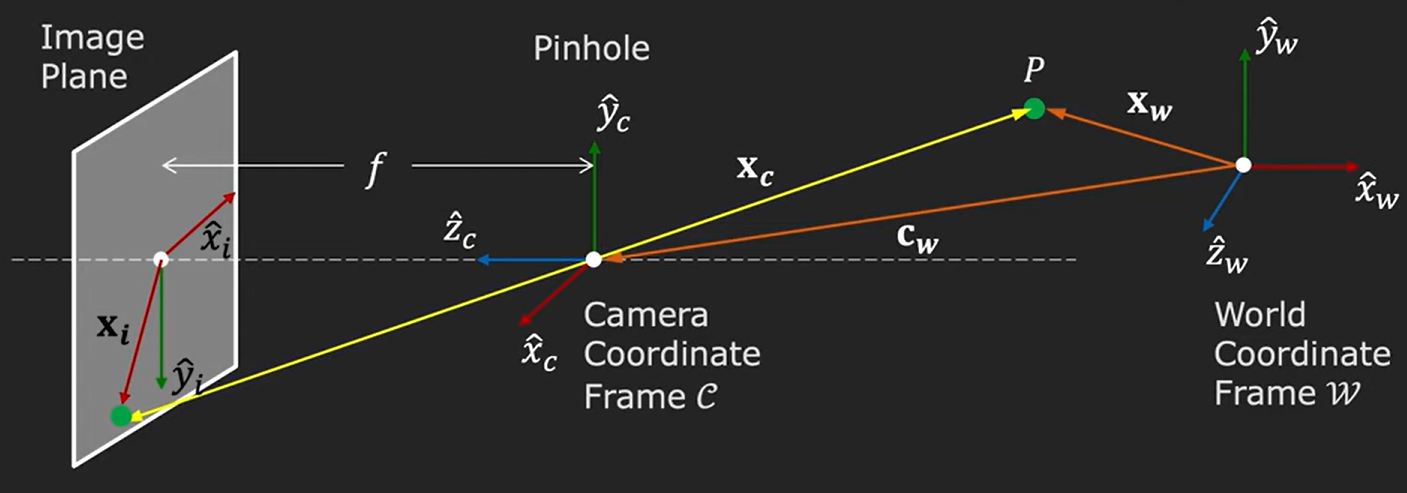
\includegraphics[width=1\textwidth]{figures/camera/forward_imaging_model.png}
    \caption{Forward imaging model of a camera. CITE}
    \label{fig:camera_forward_imaging_model}
\end{figure}

Using the forward imaging model the pixel distance was mapped to the metric distance for the x-axis with
\begin{equation}
    X = Z \times \left( \frac{x - x_{ref}}{f_x} \right)\,,
    \label{eq:pixel_to_metric}
\end{equation}
where $Z$ is the depth camera with respect to the world co-ordinate frame, $x$ is the pixel of interest, $x_{ref}$ is the reference pixel, and $f_x$ is the effective focal length of the camera. Similarly, the pixel distance was mapped to the metric distance for the y-axis.

The effective focal length of the camera $f_x$ was determined through camera calibration.

\subsubsection{Camera calibration}
\paragraph{Intrinsic parameters}\mbox{}\\
These parameters are inherent to the camera and remain constant unless the camera's internal settings (like focus) are changed. They are typically found by calibrating the camera using multiple views of a known pattern (like a checkerboard).

\begin{itemize}
    \item \textbf{Camera Matrix (K)}: Defines the camera's internal characteristics. The principal components are:
          \begin{equation}
              K = \begin{bmatrix}
                  f_x & 0   & c_x \\
                  0   & f_y & c_y \\
                  0   & 0   & 1   \\
              \end{bmatrix}
          \end{equation}\\
          where $f_x$ and $f_y$ are the focal lengths in pixels and $c_x, c_y$ are the co-ordinates of the principal point. The principal point is the pixel co-ordinate where the camera's principal axis intersects the image plane.

    \item \textbf{Distortion Coefficients (D)}: Captures lens distortion. This is a vector with up to 5 elements in the common "plumb-bob" model of OpenCV
          \[
              D = [k_1, k_2, p_1, p_2, k_3]
          \]
          where $k_1, k_2, k_3$ are radial distortion coefficients and $p_1, p_2$ are tangential distortion coefficients.
\end{itemize}

\paragraph{Extrinsic Parameters}\mbox{}\\
These parameters capture the camera's orientation and position concerning the world or an external reference frame.

\begin{itemize}
    \item \textbf{Rotation Vector (rvec)}: Represents the orientation of the camera. It's a 3x1 vector used to derive the rotation matrix $ R $.

    \item \textbf{Translation Vector (tvec)}: Represents the position of the camera. It's a 3x1 vector capturing the translation in X, Y, and Z directions.
\end{itemize}

They represent the position and orientation of the camera relative to the world (or in your case, the turret's frame). Every time you move the camera or change the scene, these parameters would change. These are found using functions like \verb|solvePnP| in OpenCV, which computes the pose of an object given some known 3D points on the object and their corresponding 2D projections in the image.

\subsubsection{Morphological operations}
\label{subsubsec:morphological_operations}
Erosion is a fundamental morphological operation used to remove small structures or details from a binary image. It is defined as the basic set operation of moving a structuring element (usually a smaller binary matrix) over the input binary image and finding the intersection of the structuring element with the image. This operation can be mathematically expressed as
\begin{equation}
    (A \ominus B)(x, y) = \bigcap \{A(x + i, y + j) | (i, j) \in B\}\,,
    \label{eq:erosion}
\end{equation}
where
\begin{itemize}
    \item $A$ is the input binary image.
    \item $B$ is the structuring element.
    \item $\ominus$ represents the erosion operation.
    \item $(x, y)$ are the pixel co-ordinates in the resulting image.
\end{itemize}

Dilation is another fundamental morphological operation, but it is used to enhance or grow the features in a binary image. Dilation can be defined as the set operation that moves the structuring element over the input image and computes the union of the element with the parts of the image where the structuring element "hits". The mathematical expression for dilation is as follows:
\begin{equation}
    (A \oplus B)(x, y) = \bigcup \{A(x + i, y + j) | (i, j) \in B\}
    \label{eq:dilation}
\end{equation}
where
\begin{itemize}
    \item $A$ is the input binary image.
    \item $B$ is the structuring element.
    \item $\oplus$ represents the dilation operation.
    \item $(x, y)$ are the pixel co-ordinates in the resulting image.
\end{itemize}

The erosion and dilation operations are illustrated in \autoref{fig:erosion_and_dilation}.
\begin{figure}[h]
    \centering
    \begin{subfigure}[t]{0.45\textwidth}
        \centering
        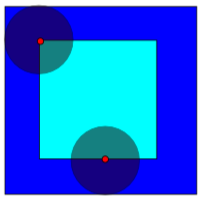
\includegraphics[width=0.5\linewidth]{figures/detection/erosion.png}
        \caption{The erosion of the dark-blue square by a disk, resulting in the light-blue square.}
        \label{fig:erosion}
    \end{subfigure}
    \quad
    \begin{subfigure}[t]{0.45\textwidth}
        \centering
        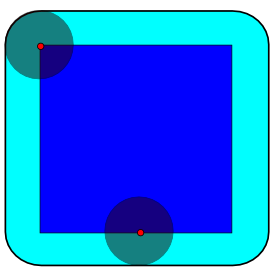
\includegraphics[width=0.5\linewidth]{figures/detection/dilation.png}
        \caption{The dilation of a dark-blue square by a disk, resulting in the light-blue square with rounded corners.}
        \label{fig:dilation}
    \end{subfigure}
    \caption{The figure shows an example of erosion and dilation. This figure was modified from Renatokeshet at the English Wikipedia (2008).}
    \label{fig:erosion_and_dilation}
\end{figure}

Opening is a compound morphological operation that consists of an erosion followed by a dilation using the same structuring element. It is primarily used to remove noise and small objects from a binary image. The opening of an image $A$ by a structuring element $B$ is defined as
\begin{equation}
    A \circ B = (A \ominus B) \oplus B\,,
    \label{eq:opening}
\end{equation}
where
\begin{itemize}
    \item $A$ is the input binary image.
    \item $B$ is the structuring element.
    \item $\circ$ represents the opening operation.
\end{itemize}

Closing is another compound morphological operation that consists of dilation followed by an erosion using the same structuring element. It is used to close small holes and gaps in objects and to connect nearby objects. The closing of an image $A$ by a structuring element $B$ is defined as
\begin{equation}
    A \bullet B = (A \oplus B) \ominus B\,,
    \label{eq:closing}
\end{equation}
where
\begin{itemize}
    \item $A$ is the input binary image.
    \item $B$ is the structuring element.
    \item $\bullet$ represents the closing operation.
\end{itemize}

Opening and closing are both idempotent operations, meaning that repeated openings or closing have no effect on the image. Opening and closing is illustrated in \autoref{fig:opening_and_closing}.
\begin{figure}[h]
    \centering
    \begin{subfigure}[t]{0.45\textwidth}
        \centering
        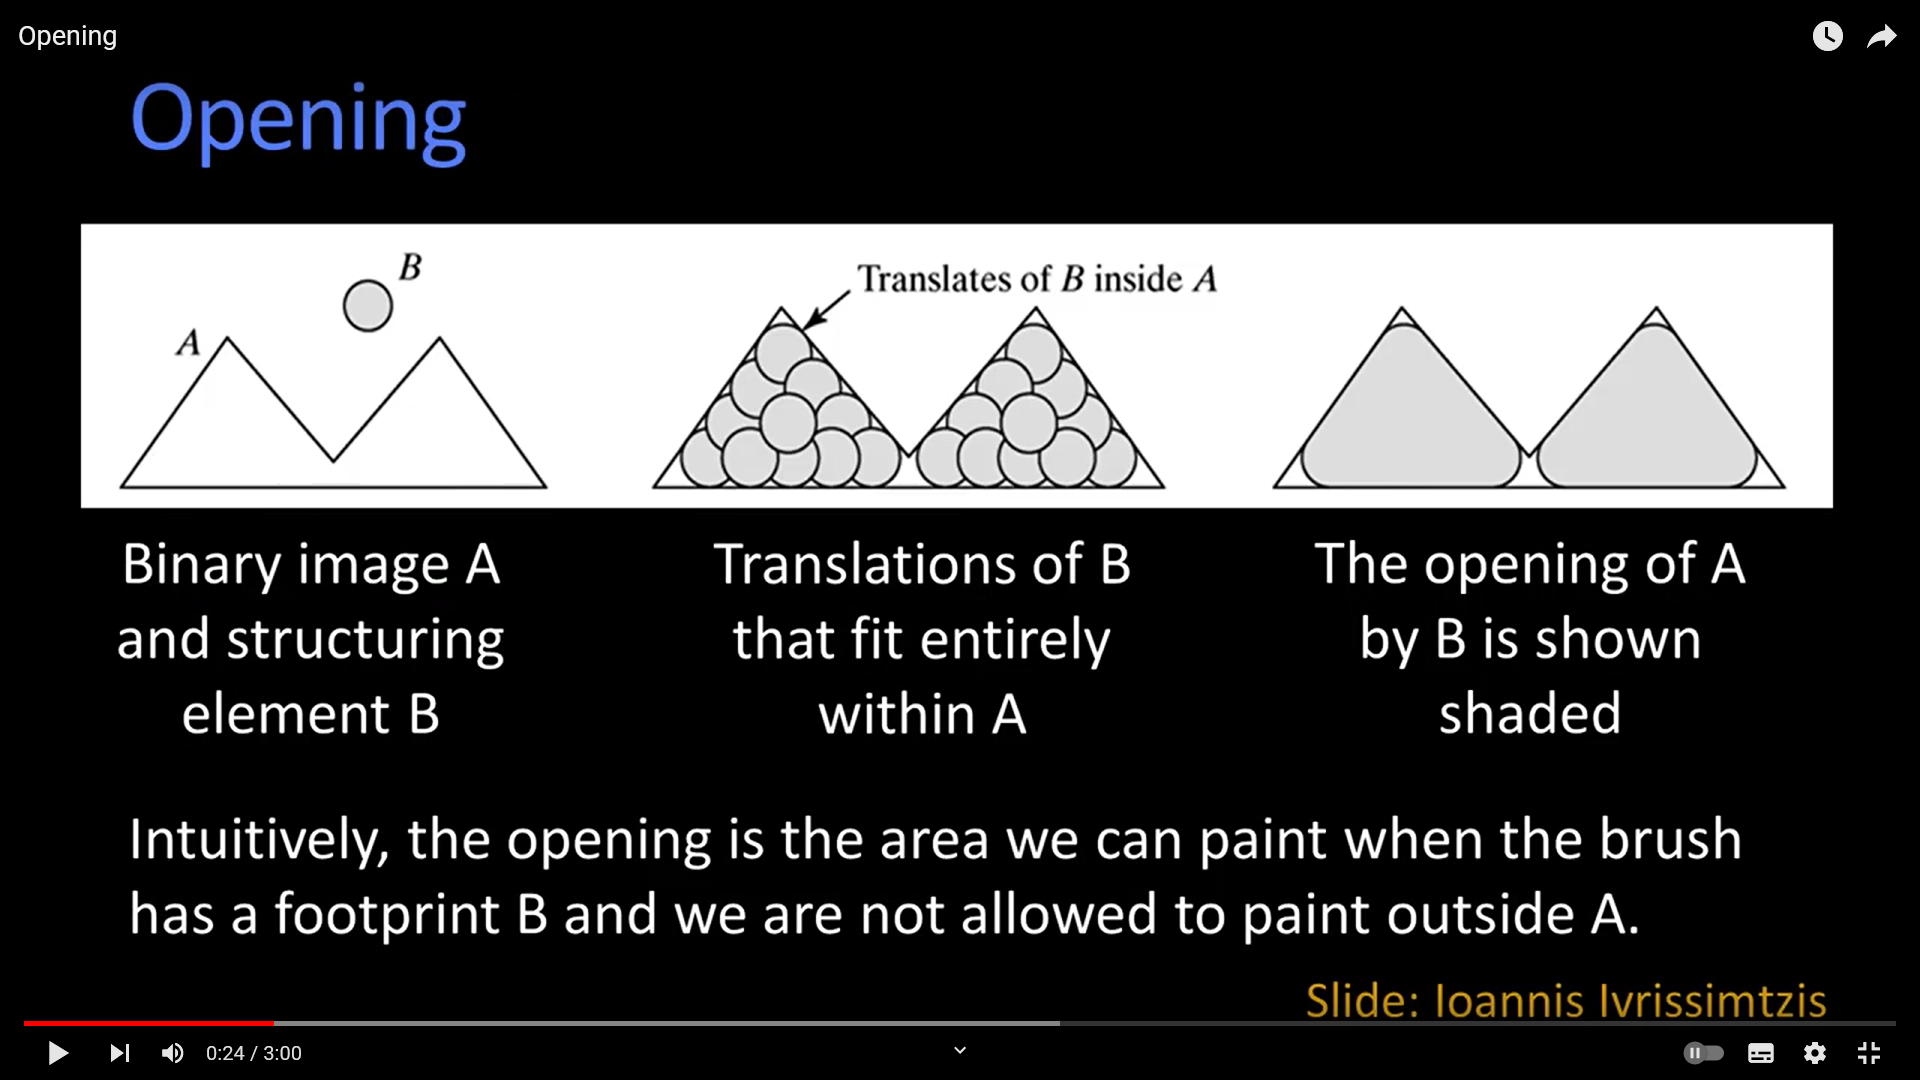
\includegraphics[width=0.5\linewidth]{figures/detection/opening.png}
        \caption{The opening of the dark-blue square by a disk, resulting in the light-blue square with round corners.}
        \label{fig:opening}
    \end{subfigure}
    \quad
    \begin{subfigure}[t]{0.45\textwidth}
        \centering
        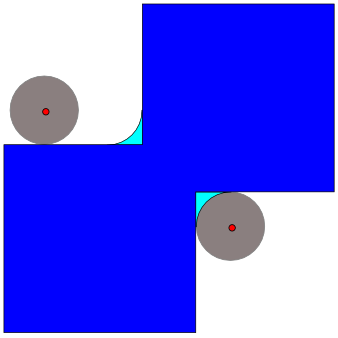
\includegraphics[width=0.5\linewidth]{figures/detection/closing.png}
        \caption{The closing of the dark-blue shape (union of two squares) by a disk, resulting in the union of the dark-blue shape and the light-blue areas.}
        \label{fig:closing}
    \end{subfigure}
    \caption{The figure shows and example of opening and closing. This figure was modified from Renatokeshet at the English Wikipedia (2008).}
    \label{fig:opening_and_closing}
\end{figure}

\subsubsection{Kalman filter} \label{subsubsec:kalman_filter}
The Kalman filter is a recursive algorithm that estimates the state of a system from a series of noisy measurements. It is a powerful tool for tracking the state of a system over time and is widely used in control systems and robotics. The Kalman filter is based on a linear dynamical system model, which is defined by the following equations:

\begin{equation}
    \begin{aligned}
        x_k & = Ax_{k - 1} + Bu_{k - 1} + w_{k - 1} \\
        z_k & = Hx_k + v_k
    \end{aligned}
    \label{eq:kalman_filter}
\end{equation}

where

\begin{itemize}
    \item $x_k$ is the state vector at time $k$.
    \item $z_k$ is the measurement vector at time $k$.
    \item $A$ is the state transition matrix.
    \item $B$ is the control matrix.
    \item $u_k$ is the control vector at time $k$.
    \item $w_k$ is the process noise vector at time $k$.
    \item $H$ is the observation matrix.
    \item $v_k$ is the measurement noise vector at time $k$.
\end{itemize}


\subsubsection{SORT tracking} \label{subsubsec:sort_tracking}
SORT (Simple Online and Realtime Tracking) is a popular algorithm for multi-object tracking in video sequences. The main goal of the SORT algorithm is to associate detection boxes across frames in a video sequence to form trajectories for each individual object. Here is a theoretical background on the SORT tracking algorithm:
1. Overview

SORT is designed to be both simple and efficient, achieving real-time performance. It is based on the tracking-by-detection paradigm, which means it relies on an external object detector to provide bounding boxes around objects of interest in each frame. The algorithm then associates these detections across frames to create tracks.
2. Detection

Before tracking, an object detection algorithm (such as Faster R-CNN, YOLO, or SSD) is applied to each frame to detect objects of interest. The output is a set of bounding boxes along with their associated confidence scores.
3. Association

The core of the SORT algorithm is the association step, where detections are linked across frames to form tracks. This is done based on the intersection over union (IoU) metric, which measures the overlap between two bounding boxes. The steps involved are:

Prediction: For each existing track, the Kalman filter is used to predict the new position of the object in the current frame.
Matching: The predicted positions of existing tracks are matched with the current frame's detections based on the IoU metric. A bipartite graph matching algorithm (such as the Hungarian algorithm) is used to find the optimal assignment.
Update: The Kalman filter for each matched track is updated with the current detection.
Creation and Deletion: New tracks are created for detections that could not be matched to existing tracks. Tracks that have not been matched for a certain number of frames are deleted.

4. Kalman Filter

The Kalman filter is a critical component of the SORT algorithm, providing a way to predict and update the state of the tracks based on the detections. The state of a track is represented as $[x,y,\dot{x},\dot{y}]$, where x,yx,y are the coordinates of the center of the bounding box, ss is the scale/area of the bounding box, rr is the aspect ratio, and $\dot{x},\dot{y}$ are the respective velocities.
5. Challenges and Limitations

Occlusions: SORT can struggle with objects that are occluded or interact closely with each other, as the IoU metric may not be sufficient for correct association.
Identity Switches: In cases where objects cross paths or are close together, SORT can suffer from identity switches.
Dependence on Detection: The performance of SORT is highly dependent on the quality of the detections provided by the external object detector.




\subsection{Simulation and Prototyping}
Detection and tracking done in python with videos.



\subsection{Hardware design}
The hardware overview is presented in \autoref{fig:hardware_overview}. The hardware consists primarily of a laser turret, a camera, a mosquito enclosure, and an embedded processing platform. The laser turret is used to move the laser beam across the mosquito enclosure. The camera is used to detect the laser beam and the mosquitoes. A bracket is used to position the laser turret and the camera relative to the mosquito enclosure. The embedded processing platform is used to control the laser turret and perform the image processing required for the laser detection and mosquito detection.
\begin{figure}[h]
    \centering
    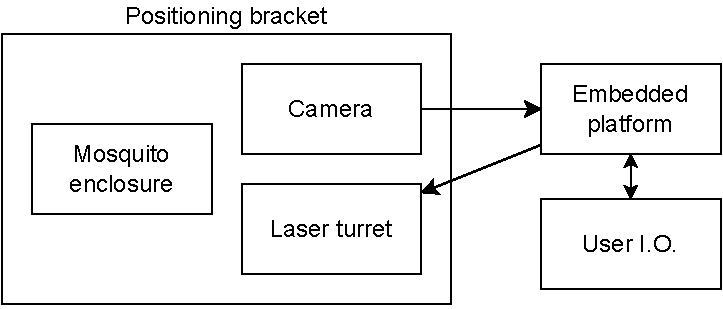
\includegraphics[width=0.75\textwidth]{figures/hardware_design/hardware_overview.pdf}
    \caption{Hardware overview.}
    \label{fig:hardware_overview}
\end{figure}



\subsubsection{Embedded platform selection}
To select an embedded platform for the project the following requirements were considered:
\begin{description}[style=nextline]
    \item[Processing power] The embedded platform must be able to perform the image processing required for the laser detection and mosquito detection in real-time. Image processing is computationally intensive, but can largely benefit from parallelisation. Therefore, an embedded platform with a \gls{gpu} will be preferred.
    \item[Memory] The embedded platform must have sufficient memory to store the multiple images along with the required algorithms. A 1080p image with 3 8-bit colour channels requires 6 MB of memory.
    \item[Hardware interfaces] The embedded platform must be compatible with camera interfaces. It must also have sufficient \gls{gpio} pins to interface with the stepper motor drivers. The embedded platform must also have support for a display output and a keyboard and mouse input to provide a user interface to control the system.
    \item[Availability and support] It is import to select an embedded platform that is readily available. It is important to select an embedded platform with large body of knowledge available and sufficient scientific support community since this is an individual project without access to people with expertise with the embedded platform.
\end{description}

The Nvidia Jetson Nano was chosen as the embedded platform for the project. The Nvidia Jetson Nano is a single-board computer with a \gls{gpu} and a quad-core \gls{cpu}. The Nvidia Jetson Nano has a \gls{mipi} \gls{csi}-2 camera interface and has 40 \gls{gpio} pins. The Jetson Nano has a quad-core ARM Cortex-A57 MPCore processor, an Nvidia Maxwell \gls{gpu} with 128 \gls{cuda} cores, and 4 GB of LPDDR4 memory. It also features an HDMI display output and a \gls{usb} 3.0 port. The Nvidia Jetson Nano is readily available and has a large body of knowledge available and sufficient scientific support community.



\subsubsection{Camera selection}
To minimise the computational complexity of the image processing required for the laser detection and mosquito detection a low resolution will be used. The video resolution will not need to exceed 1080p. The camera must be able to capture images at a frame rate of at least 30 frames per second. The camera must also be compatible with the \gls{mipi} \gls{csi} on the Nvidia Jetson Nano.

The Raspberry Pi Camera Module V2 was chosen as the camera for the project. The Raspberry Pi Camera Module V2 is an 8 MP camera that can capture images at a frame rate of 30 frames per second at 1080p. The Raspberry Pi Camera Module V2 is compatible with the \gls{mipi} \gls{csi} on the Nvidia Jetson Nano.



\subsubsection{Mosquito enclosure}
The mosquito enclosure will be a rectangular prism as shown in \autoref{fig:mosquito_enclosure_dimensions}. The width of the enclosure must be a minimum length of 1 metre. The front facing surface will be transparent and the rest of the surfaces will be white. The enclosure will be fitted with internal lighting to ensure contrast between the background and the mosquitoes and to minimise the camera noise.
\begin{figure}[h]
    \centering
    % 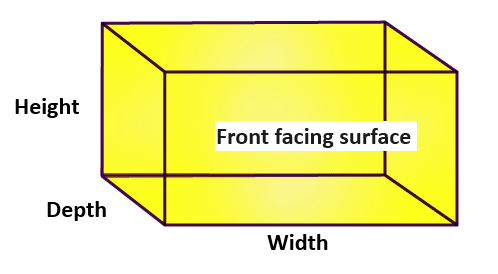
\includegraphics[width=0.5\textwidth]{figures/hardware_design/rectangular_prism.png}
    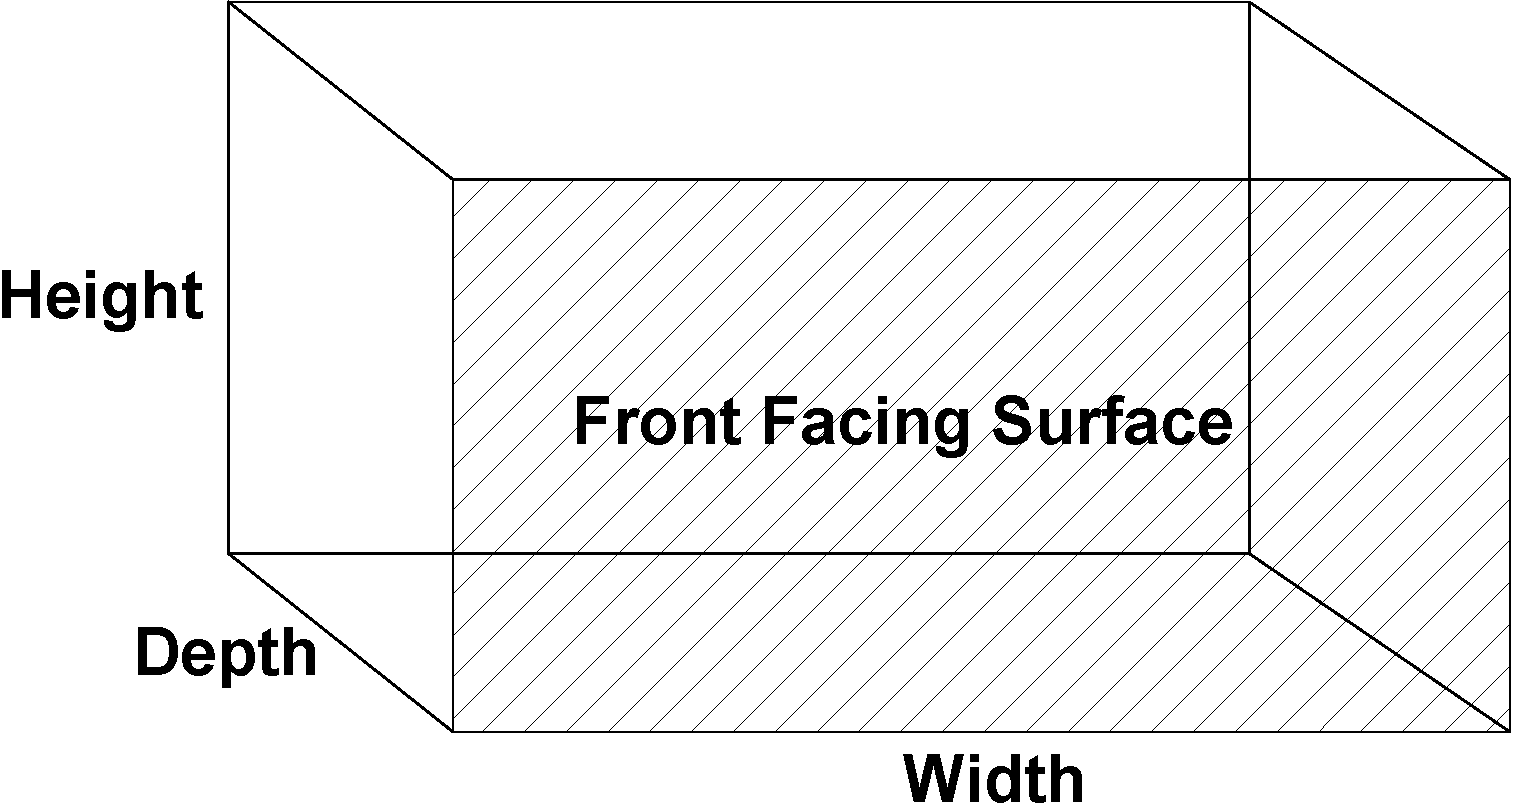
\includegraphics[width=0.7\textwidth]{figures/hardware_design/mos_enclosure.pdf}
    \caption{Mosquito enclosure dimensions.}
    \label{fig:mosquito_enclosure_dimensions}
\end{figure}



\subsubsection{System positioning}\label{subsubsec:system_positioning}
The laser turret and the camera will be placed outside the mosquito enclosure in known positions relative to the enclosure. The bracket, shown in \autoref{fig:system_positioning_bracket}, will be built to hold the laser turret and the camera in place relative to the mosquito enclosure.
\begin{figure}[h]
    \centering
    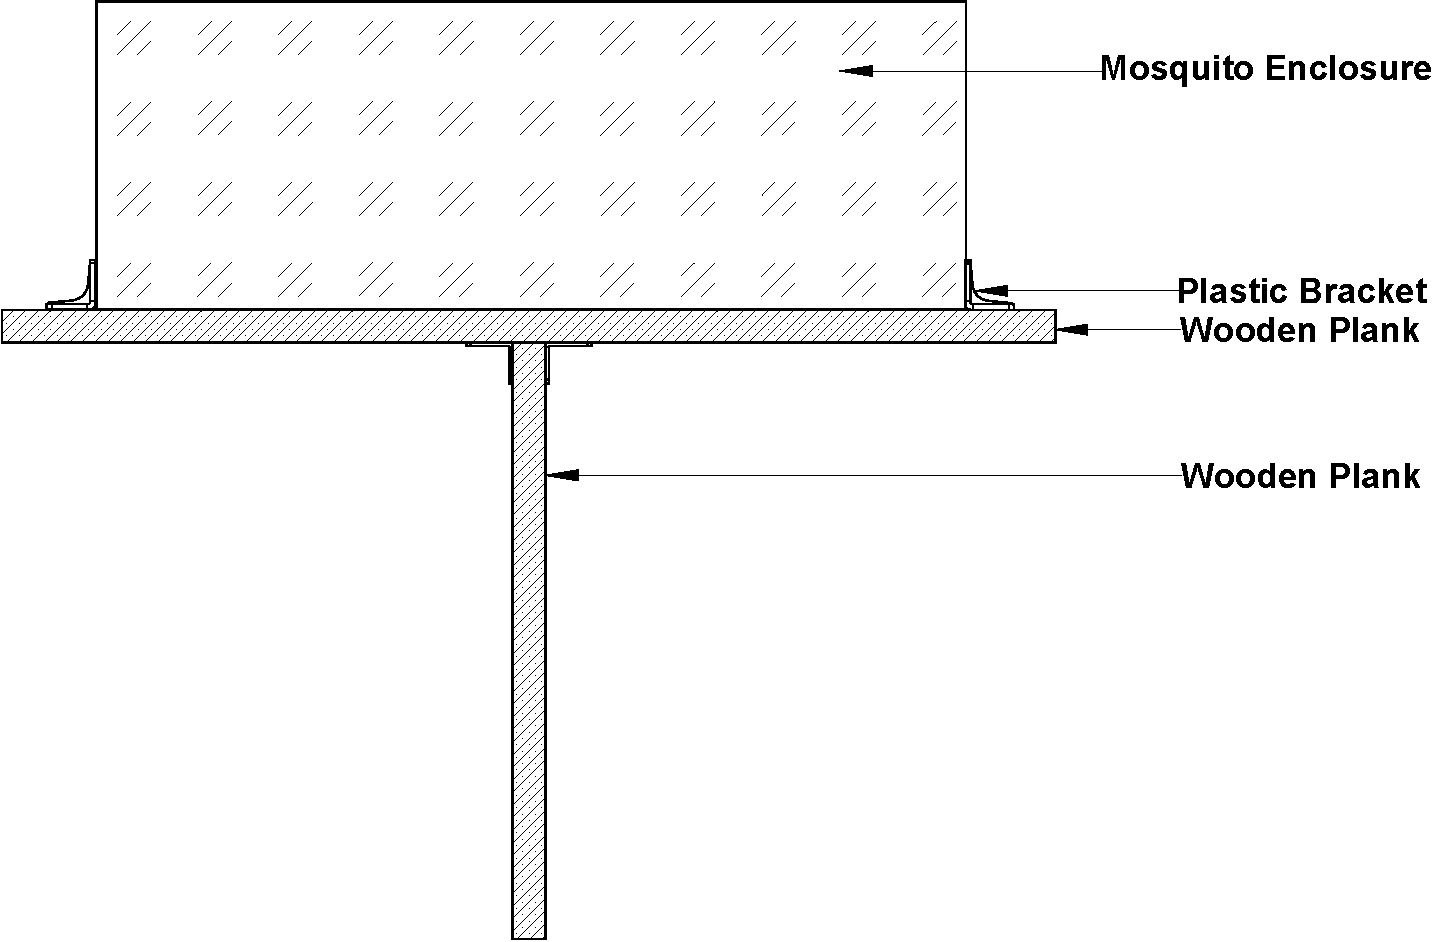
\includegraphics[width=1\textwidth]{figures/hardware_design/system_positioning.pdf}
    \caption{System positioning bracket.}
    \label{fig:system_positioning_bracket}
\end{figure}



\subsubsection{Laser turret}\label{subsubsec:laser_turret_design}
The laser turret design was inspired by commercial two-axis laser scanners. The position of the laser beam is controlled by adjusting the angles of two mirrors. This is illustrated in \autoref{fig:two-axis-scanner-schematic}. The mirrors are connected directly to the output shaft of the motors. The laser turret will be positioned orthogonally to the $xy$-plane of the mosquito enclosure. The point where the laser beam shines orthogonal to the $xy$-plane of the mosquito enclosure is considered the origin of the laser. This will occur when the two mirrors are at 45$\degree$ relative to the laser beam.
\begin{figure}[h]
    \centering
    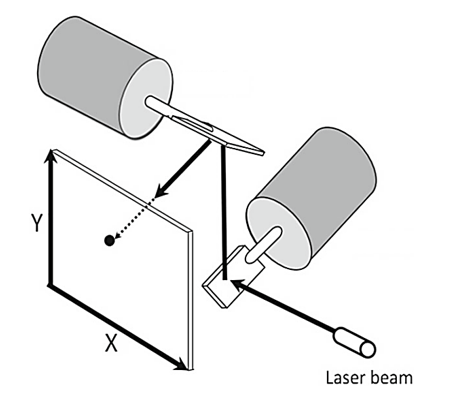
\includegraphics[width=0.5\textwidth]{figures/hardware_design/two_axis_scanner.png}
    \caption{Two-axis laser scanner schematic. This figure was modified from \cite{two-axis-scanner-schematic}.}
    \label{fig:two-axis-scanner-schematic}
\end{figure}

When a single axis of the laser turret is considered it can be seen that a right triangle is formed between the laser turret and the $xy$-plane mosquito enclosure as shown in \autoref{fig:mirror_angle}. Using the properties of a right triangle the mirror angle $\theta$ required to shine the laser a distance $d$ relative to the origin of the laser can be calculated using
\begin{equation}
    \theta = \arctan{\left(\frac{d}{z}\right)}\,,
    \label{eq:mirror_angle}
\end{equation}
where $z$ is the distance between the turret and the back wall of the mosquito enclosure.
\begin{figure}[h]
    \centering
    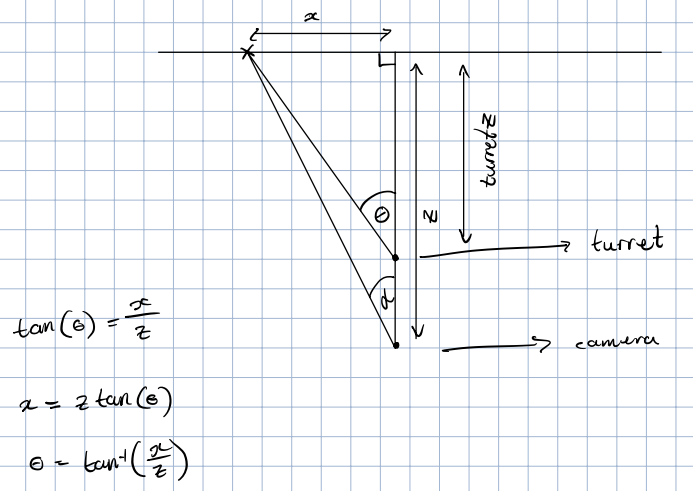
\includegraphics[width=0.5\textwidth]{figures/hardware_design/mirror_angle.png}
    \caption{Mirror angle calculation.}
    \label{fig:mirror_angle}
\end{figure}

\newcommand{\requiredLatStepSizeMM}{2}
The lateral step size of the laser must be a maximum of $\requiredLatStepSizeMM$\,mm. This will ensure that the laser will be able to illuminate every position in the mosquito enclosure since the laser itself will be a few millimetres wide.

\newcommand{\requiredLatSpeedMPS}{1}
The required lateral speed is determined in accordance with the field specifications. The longest length of the mosquito enclosure $d_{max}$ will be $\SI{1}{\meter}$. To ensure that the laser can illuminate any set point inside the mosquito enclosure within $\SI{2}{\second}$ of receiving a step input, it was assumed that the laser must be able to move with a velocity $v_{laser}$ of least $\SI{\requiredLatSpeedMPS}{\meter\per\second}$ opposed to the $\SI{0.5}{\meter\per\second}$ required to move the $\SI{1}{\meter}$ length of the mosquito enclosure within $\SI{2}{\second}$. This was done to accommodate for the settling time of the laser turret control system.




\subsection{Hardware implementation}



\subsubsection{Mosquito enclosure}
\newcommand{\enclosureWidthCM}{90} % cm
\newcommand{\enclosureHeightCM}{38} % cm
\newcommand{\enclosureDepthCM}{32} % cm

The mosquito enclosure was constructed from a second hand glass fish tank with dimensions $\enclosureWidthCM \times \enclosureHeightCM \times \enclosureDepthCM$ cm. All the surfaces other than front facing surface was retrofitted with a white lining. Internal \glspl{led} were added to the enclosure, shining from the top and bottom surfaces to minimise shadows on the back surface the enclosure, to ensure contrast between the background and the mosquitoes and to minimise the camera noise.



\subsubsection{Laser turret}
The specific geometry of the laser turret was designed with the goal to practically obtain a sufficiently small lateral step size of the laser on the back wall of the mosquito enclosure, while maintaining sufficient speed. The dimensions of the mirrors were chosen for practicality as $30 \times 15 \times 3$~mm.


\label{par:angular_step_size}
\paragraph{Angular step size}\mbox{}\\
The turret axis on which the laser beam is first incident on will be referred to as the first axis and the other axis will be referred to as the second axis for the remainder of this discussion. The rotation range of the first axis is bounded by the geometry of the turret since the laser beam reflected from the first axis must be incident on the second axis. With the chosen mirror dimensions, the maximum angle through which the first axis can rotate is $40\degree$. This was conservatively determined geometrically in the to scale drawing in \autoref{fig:turret_motion_range}. The rotation range of the second axis is not bounded by the geometry of the laser turret since the laser beam reflected from the second axis is incident on the mosquito enclosure. Therefore, the laser turret will be oriented such that the first axis moves the laser beam parallel to the shorter width of the mosquito enclosure and the second axis moves the laser beam parallel to the longer length of the mosquito enclosure.
\begin{figure}[h]
    \centering
    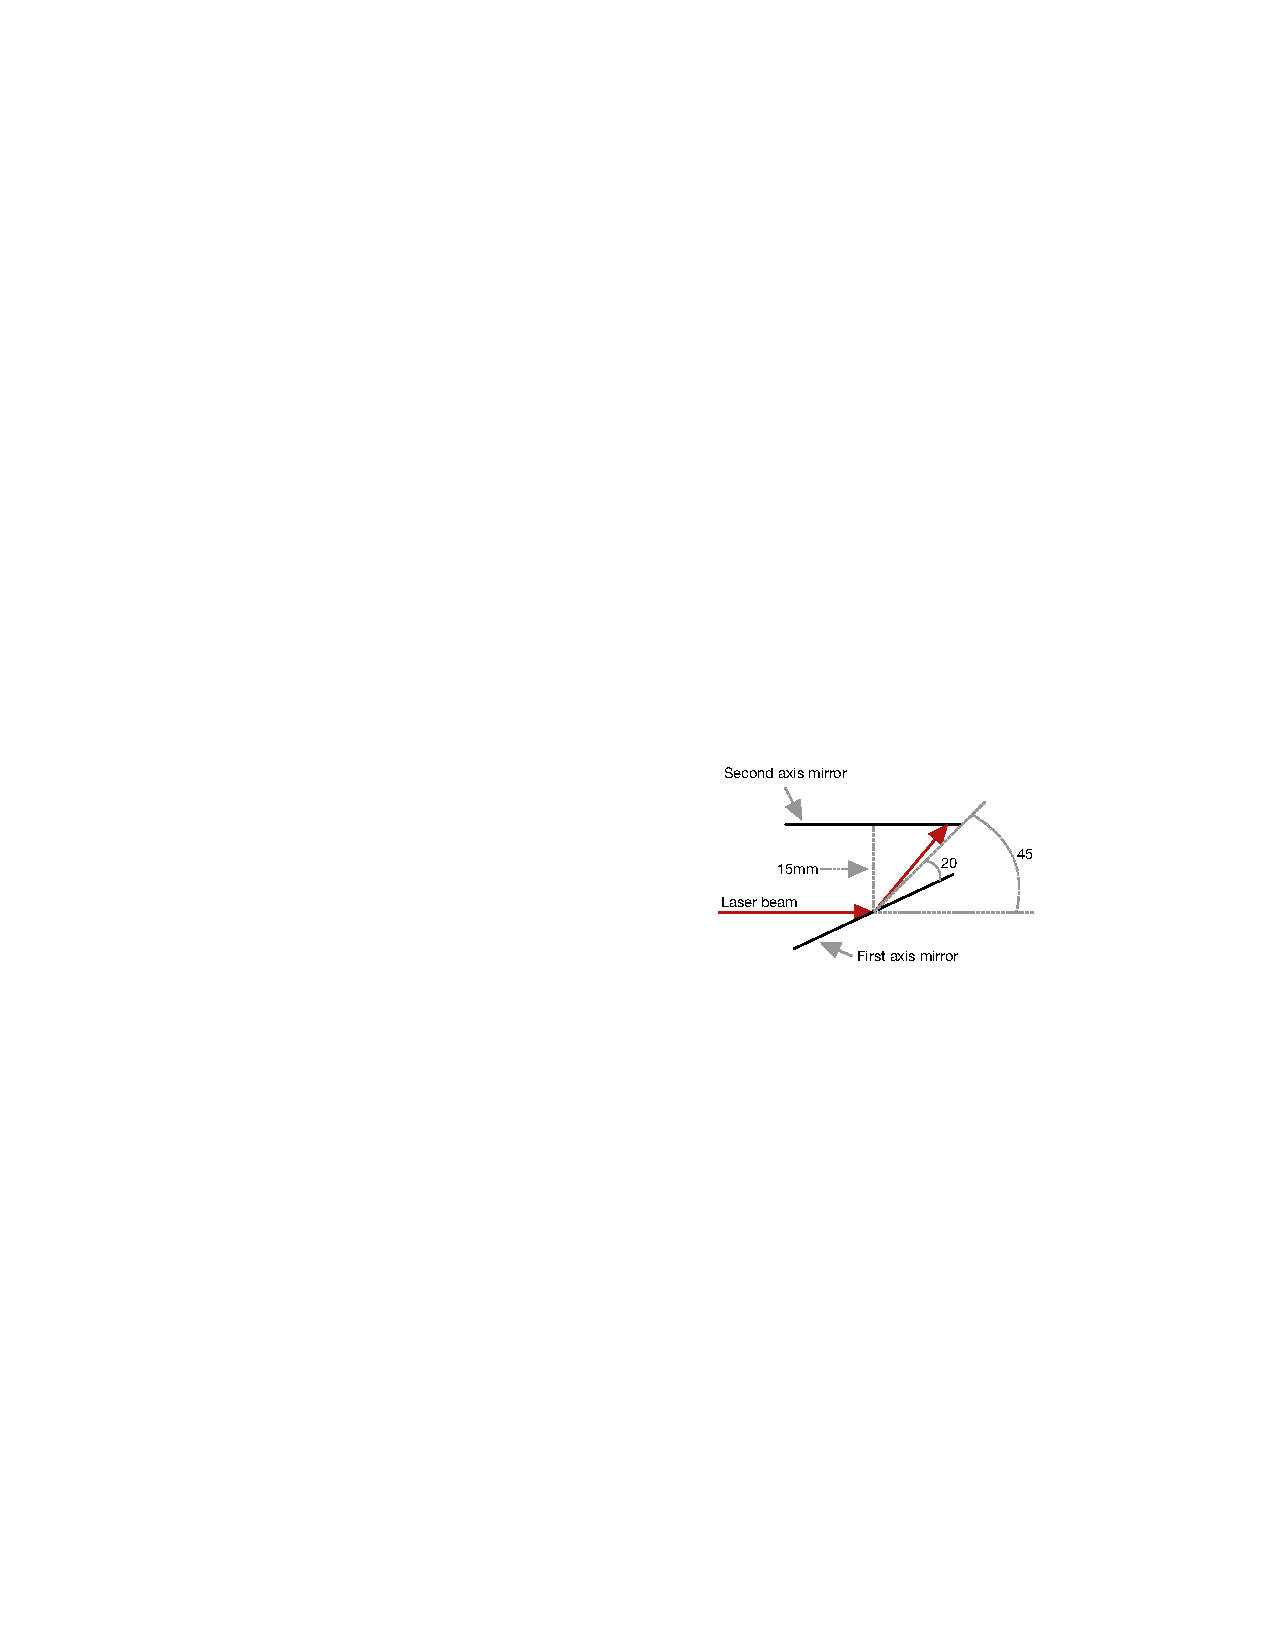
\includegraphics[width=0.6\textwidth]{figures/hardware_design/rotation_range_of_first_axis.pdf}
    \caption{Rotation range of first axis with chosen mirror dimensions.}
    \label{fig:turret_motion_range}
\end{figure}

The minimum distance $z_{min}$ between the laser turret and the mosquito enclosure can be determined by rearranging \autoref{eq:mirror_angle} to give
\FPeval{\zMinCM}{round(\enclosureHeightCM/tan(40*pi/180), 1)}
\begin{equation}
    z_{min} = \frac{d}{\tan\left(\theta\right)} = \frac{\enclosureHeightCM \text{ cm}}{\tan\left(40\degree\right)} = \zMinCM \text{ cm}\,,
\end{equation}
where $d = \enclosureHeightCM$~cm is the height of the mosquito enclosure and $\theta = 40\degree$ is the maximum angle through which the first axis of the laser turret can rotate. The maximum step resolution $\theta_{step}^{max}$ of the motors can be calculated by substituting $z_{min}$ and the required lateral step size $d_{min}$ into \autoref{eq:mirror_angle} to produce
\pgfmathsetmacro{\stepRes}{atan2(\requiredLatStepSizeMM, \zMinCM*10)}
\begin{equation}
    \theta_{step}^{max} = \arctan\left({\frac{x_{min}}{z_{min}}}\right) = \arctan\left({\frac{\requiredLatStepSizeMM \text{mm}}{\zMinCM \text{cm}}}\right) = \FPeval{\roundStepRes}{round(\stepRes, 3)}\roundStepRes\degree\,.
    \label{eq:max_step_resolution}
\end{equation}


\paragraph{Angular speed}\mbox{}\\
The maximum angular speed $\omega_{max}$ required by the motors can be determined with $d_{max}$, $v_{laser}$, and $z_{min}$. The maximum angle through which the turret must rotate is
\begin{equation}
    \theta_{max} = \arctan\left({\frac{d_{max}}{z_{min}}}\right) = \arctan\left({\frac{\SI{1}{\meter}}{\zMinCM \text{ cm}}}\right) = 65.6\degree\,.
\end{equation}
The maximum angular speed required to move the laser beam at the lateral speed $v_{laser} = \SI{\requiredLatSpeedMPS}{\meter\per\second}$ is
\begin{equation}
    \omega_{max} = v_{laser} \times \theta_{max} = \SI{65.6}{\degree\per\second} = \SI{1.14}{\radian\per\second}\,.
\end{equation}
The results in a required motor \gls{rpm} of
\begin{equation}
    \omega_{max} = \frac{1}{2\pi} \times \SI{1.14}{\radian\per\second} \times \frac{60}{1} = 10.9 \text{ RPM}\,.
\end{equation}


\paragraph{Torque}\hfill\\
The required torque $\tau$ was calculated using
\begin{equation}
    \tau = I\alpha\,,
    \label{eq:torque}
\end{equation}
where $I$ is the moment of inertia of the load, which is the mirror, and $\alpha$ is the required angular acceleration.

\begin{figure}[h]
    \centering
    % 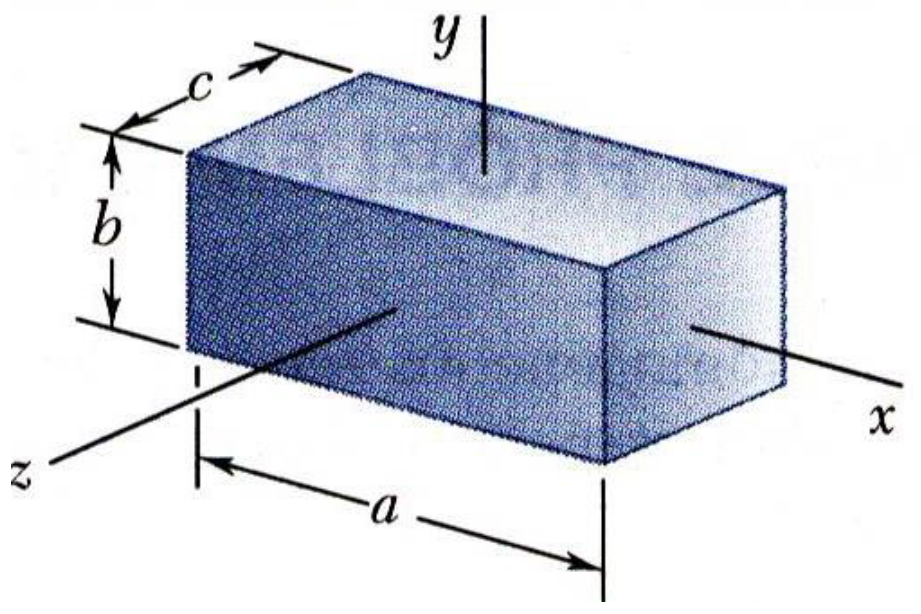
\includegraphics[width=0.5\textwidth]{figures/hardware_design/rect_inertia.png}
    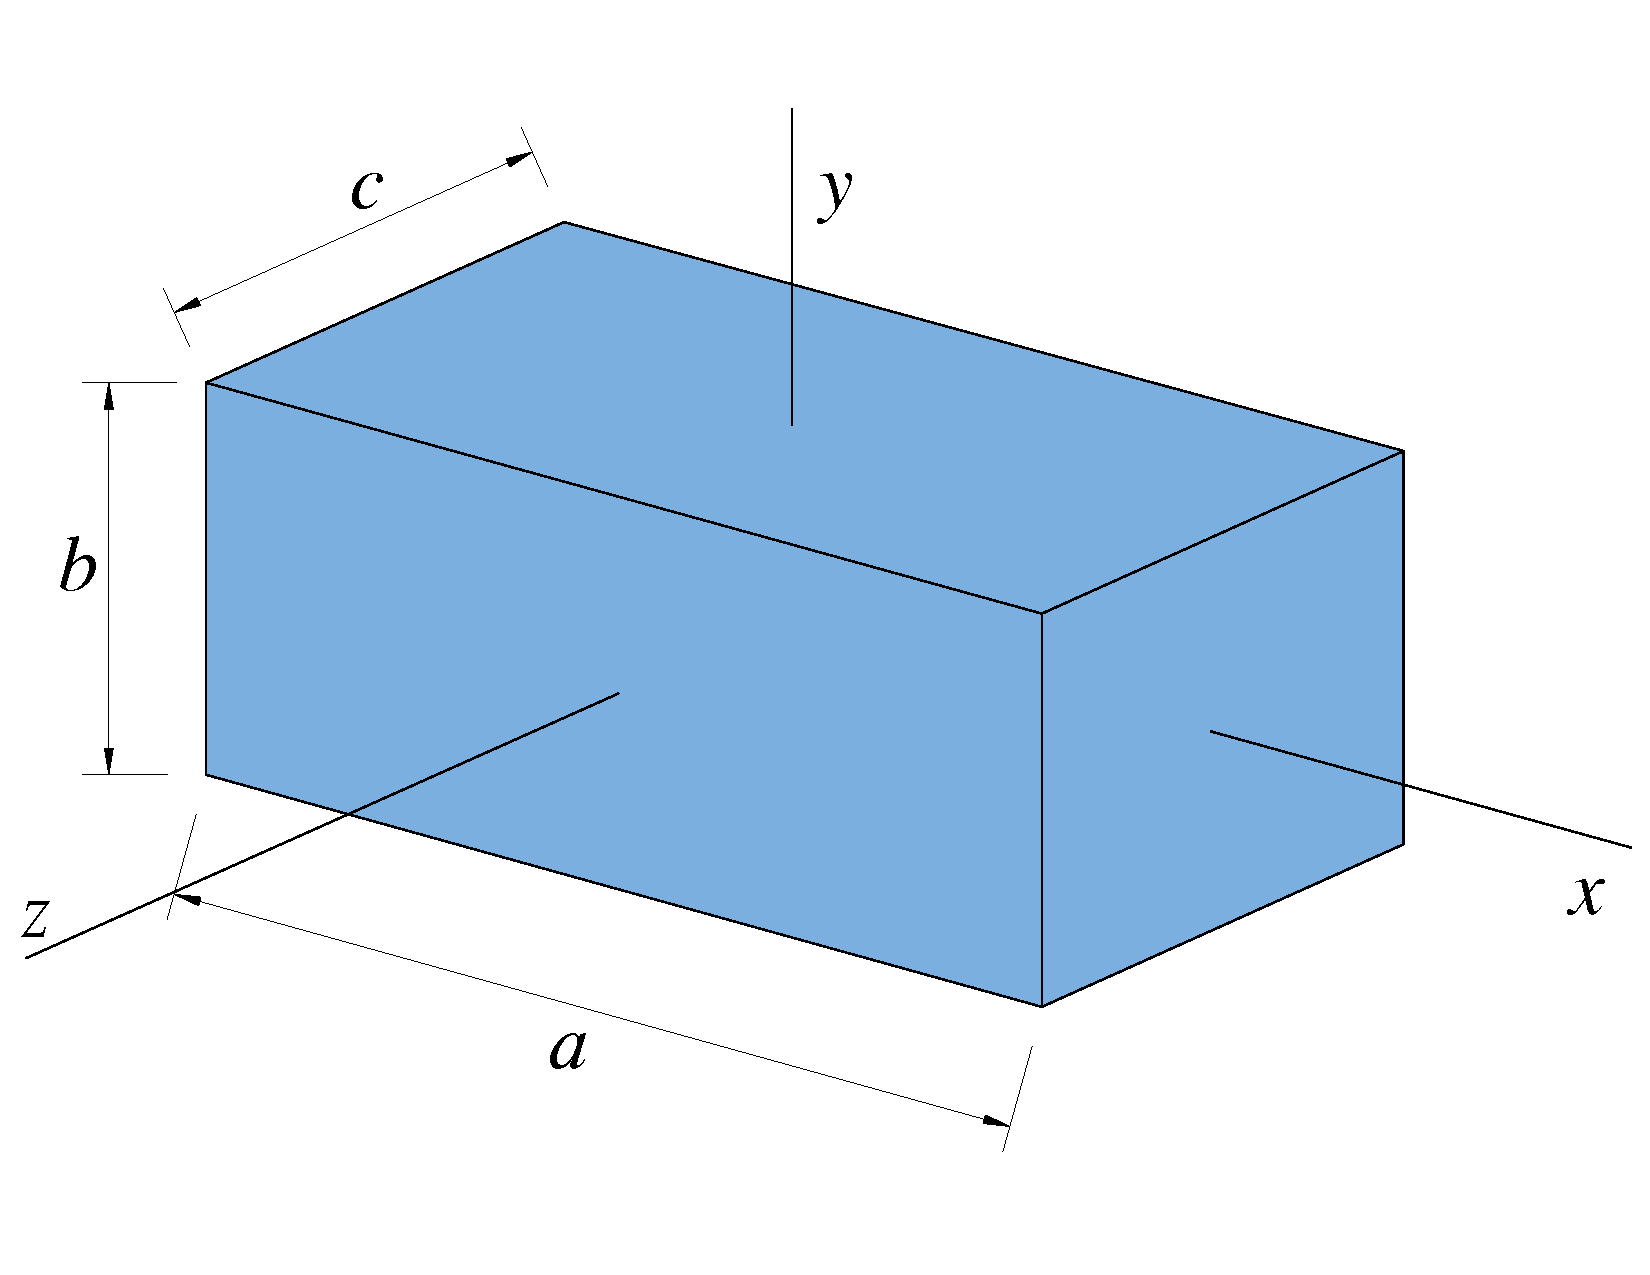
\includegraphics[width=0.6\textwidth]{figures/hardware_design/inertia_of_rectangle.pdf}
    \caption{Axes and dimensions of a rectangular prism.}
    \label{fig:rect_inertia}
\end{figure}
The moment of inertia of the mirror was calculated using the equation for the moment of inertia of a rectangular prism with rotation about its $x$-axis as seen in \autoref{fig:rect_inertia} given by
\begin{equation}
    I = \frac{1}{12}M\left(b^2 + c^2\right)\,,
\end{equation}
where $M$ is the mass of the rectangular prism and $b$ and $c$ are the dimensions of the rectangular prism. The mass of the rectangular prism $M$ will be calculated using the density of glass $\rho = \SI{2500}{\kg\per\meter\cubed}$ and the volume of the rectangular prism $V$ given by
\begin{equation}
    V = abc\,,
\end{equation}
where $a$, $b$, and $c$ are the dimensions of the rectangular prism. The dimensions of the rectangular prism is given by the chosen mirror dimensions as $a = 30\,\text{mm}$, $b = 15\,\text{mm}$, and $c = 3\,\text{mm}$. The mass of the mirror $M$ is
\begin{equation}
    M = \rho V = \SI{2500}{\kg\per\meter\cubed} \times (30\,\text{mm})(15\,\text{mm})(3\,\text{mm}) = 3.38\,\text{g}\,.
\end{equation}
Thus, the moment of inertia of the mirror is
\begin{equation}
    I = \frac{1}{12}M\left(b^2 + c^2\right) = \frac{1}{12}(3.38\,\text{g})\left((15\,\text{mm})^2 + (3\,\text{mm})^2\right) = \SI{6.59e-8}{\kg\per\meter\squared}\,.
\end{equation}

The required angular acceleration of the motor $\alpha$ is calculated with
\begin{equation}
    \alpha = \frac{\Delta\omega}{\Delta t}\,,
\end{equation}
where $\Delta\omega = \omega_{max} - 0$ is the change in angular velocity and $\Delta t$ is the change in time. The change in time $\Delta t$ was determined by assuming the laser must be able to accelerate from a stand still to $v_{laser} = \SI{1}{\meter\per\second}$ extremely rapidly to ensure that the motors could respond to the irregular flight pattern of a mosquito. It was assumed that this acceleration must occur within 10~ms. Thus, the required angular acceleration $\alpha$ is
\begin{equation}
    \alpha = \frac{\Delta\omega}{\Delta t} = \frac{\SI{1.14}{\radian\per\second}}{\SI{0.01}{\second}} = \SI{114}{\radian\per\second\squared}\,.
\end{equation}

Given the calculated moment of inertia and angular acceleration the required torque $\tau$ is
\begin{equation}
    \tau = I\alpha = \SI{6.59e-8}{\kg\per\meter\squared} \times \SI{114}{\radian\per\second\squared} = \SI{7.51e-6}{\newton\meter}\,.
\end{equation}


\paragraph{Motor and driver selection}\hfill\\
Typical stepper motors have a basic step angle of $1.8\degree$. This does not meat the required step resolution $\theta_{step}^{max} = 0.253\degree$, however the step angle can be reduced by using microstepping. Microstepping works by interpolating the \gls{pwm} signal to the stepper motor driver to produce intermediate step positions between the basic step positions. Stepper motor drivers that support up to 16 microsteps are readily available. Drivers that support up to 256 microsteps are also available. The step angle $\theta_{step}$ of a stepper motor using 8 microsteps is
\begin{equation}
    \theta_{step} = \frac{1.8\degree}{16} = 0.1125\degree\,,
\end{equation}
which is sufficient to meet the maximum required step resolution $\theta_{step}^{max} = 0.253\degree$. Therefore, a typical stepper motor with a basic step angle of $1.8\degree$ operated using at least 8 microsteps will be sufficient.

A drawback of using microstepping is that the effective torque of the stepper motor is reduced with each increase in microstepping. The torque reduction due to microstepping can be calculated with
\begin{equation}
    \tau_{eff} = \tau_{rated} \sin \left(\frac{\pi S}{2}\right)\,,
\end{equation}
where
\begin{itemize}
    \item $\tau_{eff}$ is the effective torque of the stepper motor for a specific amount of microstepping.
    \item $\tau_{rated}$ is the rated torque of the stepper motor.
    \item $S$ is the reciprocal of the number of microsteps.
\end{itemize}

The effective torque of a stepper motor for the full range of microsteps available is tabulated in \autoref{tab:effective_torque}. It can be seen that microstepping has a drastic impact of the effective torque of the stepper motor. Thus, the required torque will need to be calculated for the chosen microstepping operation.
\begin{table}[h]
    \centering
    \begin{tabular}{|c|c|}
        \hline
        Microsteps & Effective torque \\
        \hline
        1          & 100\%            \\
        2          & 70.71\%          \\
        4          & 38.27\%          \\
        8          & 19.51\%          \\
        16         & 9.8\%            \\
        32         & 4.91\%           \\
        64         & 2.45\%           \\
        128        & 1.23\%           \\
        256        & 0.61\%           \\
        \hline
    \end{tabular}
    \caption{Effective torque of stepper motor for full range of microsteps.}
    \label{tab:effective_torque}
\end{table}

The DRV8825 stepper motor driver was chosen since it is readily available and supports up to 32 microsteps. The DRV8825 stepper motor driver has a maximum current rating of 2.5~A and a maximum voltage rating of 45~V. The maximum microstepping mode will be utilised for increased resolution in the control of the laser. The required torque with 32 microsteps is
\begin{equation}
    \tau_{required} = \SI{7.51e-6}{\newton\meter} \times \frac{100\%}{4.91\%} = \SI{1.53e-4}{\newton\meter}\,.
\end{equation}

A bipolar NEMA8 stepper motor with specifications shown in \autoref{tab:nema8_specs}
\begin{table}[h]
    \centering
    \begin{tabular}{rl}
        Basic step angle & $\SI{1.8}{\degree}$                               \\
        Holding torque   & $180\,\text{g\,cm} = \SI{1.77e-2}{\newton\meter}$ \\
        Rated voltage    & 3.9~V                                             \\
        Rated current    & 0.6~A                                             \\
    \end{tabular}
    \caption{Specifications of the NEMA8 stepper motor.}
    \label{tab:nema8_specs}
\end{table}
\begin{figure}[h]
    \centering
    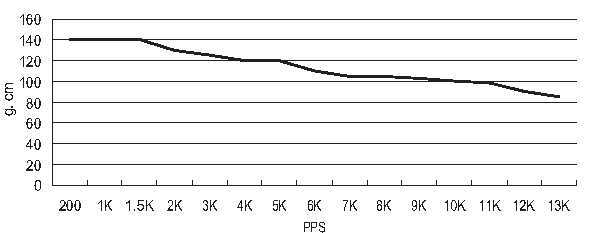
\includegraphics[width=\textwidth]{figures/hardware_design/torque_curve.pdf}
    \caption{Pull-out torque curve of the stepper motor at half step with 24~V and 0.6~A.}
    \label{fig:torque_curve}
\end{figure}
and a pull-out torque curve at half step shown in \autoref{fig:torque_curve} was chosen as the motors for the laser turret. From the pull-out torque curve in \autoref{fig:torque_curve}, the maximum rated speed of the motor is given as 13\,000 points per second at half step $0.9\degree$ which is
\begin{equation}
    \num{13000} \div \frac{360}{0.9} = 32.5\,\text{RPM}\,,
\end{equation}
with a pull-out torque greater than 100\,g\,cm = $\SI{9.8e-3}{\newton\meter}
$. The effective torque of the stepper motor at maximum speed with 32 microsteps is
\begin{equation}
    \tau_{eff} = \SI{9.8e-3}{\newton\meter} \times 4.91\% = \SI{4.81e-4}{\newton\meter}\,.
\end{equation}
The effective torque of the stepper motor at maximum speed is greater than the required torque for the laser turret, therefore the NEMA8 stepper motor is suitable for the laser turret and was also chosen for its compactness which can be seen in \autoref{fig:nema8_dimensions}.
\begin{figure}[h]
    \centering
    \begin{subfigure}{0.45\textwidth}
        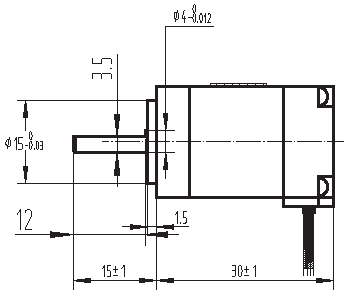
\includegraphics[width=\linewidth]{figures/hardware_design/nema8_side_view.pdf}
        \caption{Side view.}
    \end{subfigure}
    \quad
    \begin{subfigure}{0.45\textwidth}
        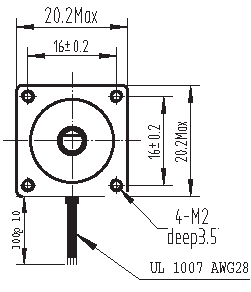
\includegraphics[width=\linewidth]{figures/hardware_design/nema8_front_view.pdf}
        \caption{Front view.}
    \end{subfigure}
    \caption{Dimensions of the NEMA8 stepper motor.}
    \label{fig:nema8_dimensions}
\end{figure}


\paragraph{Laser selection and activation circuit}\hfill\\
A low-powered 5~mW red laser with adjustable focus was chosen for the laser turret. The laser has an operating voltage range of $2.8 - 5.2$\,V. A low-powered laser was chosen for safety. The adjustable focus enabled the laser beam to be focused to a small spot size on the back wall of the mosquito enclosure. The laser must be red since the image processing will be done using on the red channel of the \gls{rgb} video frame.

The 3.3~V \gls{gpio} of the Nvidia Jetson Nano cannot supply enough current to power the laser. A transistor circuit was designed to enable the laser to be turned on and off from the Nvidia Jetson Nano \gls{gpio}.


\paragraph{Laser turret \gls{cad}}
The laser turret was designed in \gls{cad} using Autodesk Fusion 360. The laser turret was designed to be mounted on the bracket shown in \autoref{fig:system_positioning_bracket}. The main component and subcomponents of the laser turret can be seen in \autoref{fig:turret_cad} and \autoref{fig:turret_subcomponents} respectively.
\begin{figure}[!htb]
    \centering
    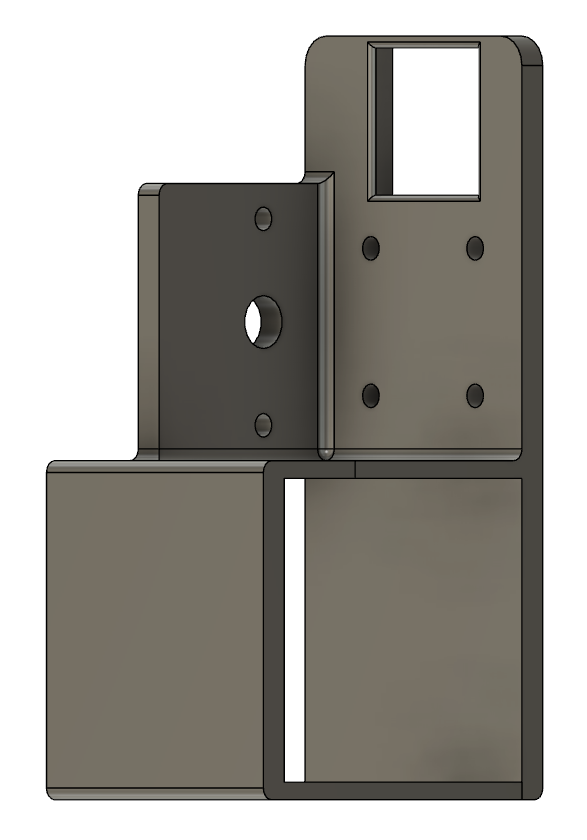
\includegraphics[width=0.4\textwidth]{figures/hardware_design/turret.png}
    \caption{Laser turret main component.}
    \label{fig:turret_cad}
\end{figure}
\begin{figure}[!htb]
    \centering
    \begin{subfigure}{0.45\textwidth}
        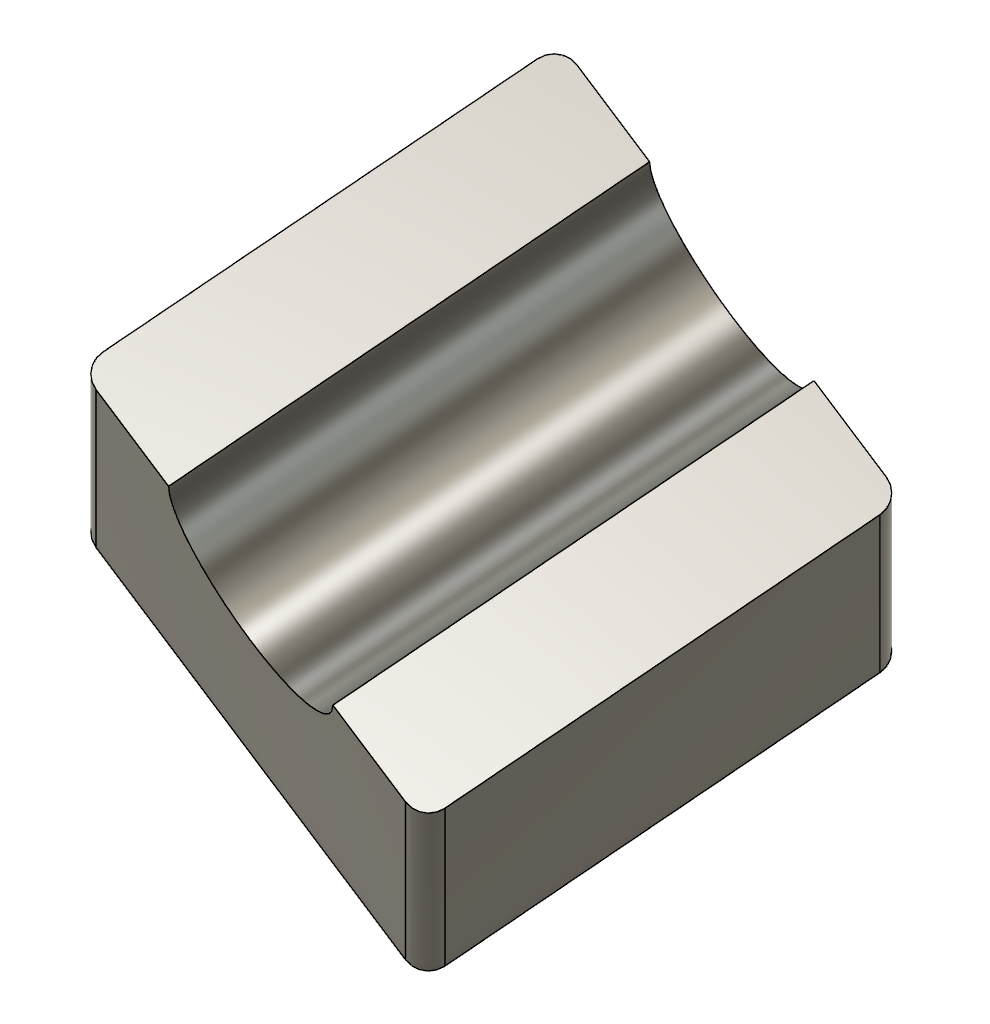
\includegraphics[width=0.8\linewidth]{figures/hardware_design/laser_mount.png}
        \caption{Laser mount.}
    \end{subfigure}
    \quad
    \begin{subfigure}{0.45\textwidth}
        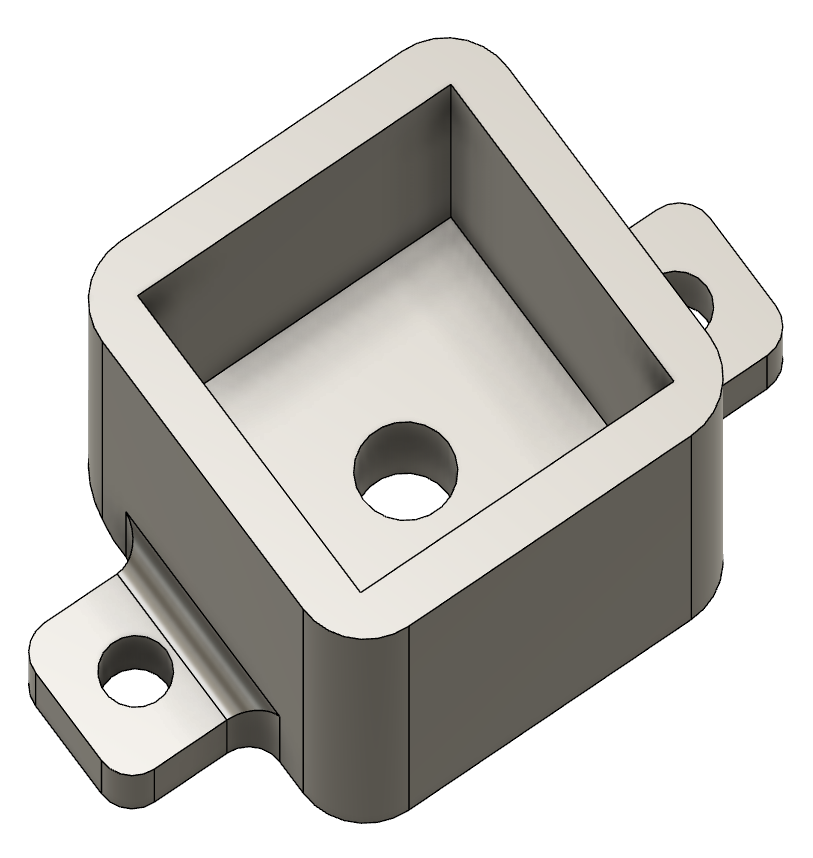
\includegraphics[width=0.8\linewidth]{figures/hardware_design/motor_mount.png}
        \caption{Motor mount.}
    \end{subfigure}
    \quad
    \begin{subfigure}{0.45\textwidth}
        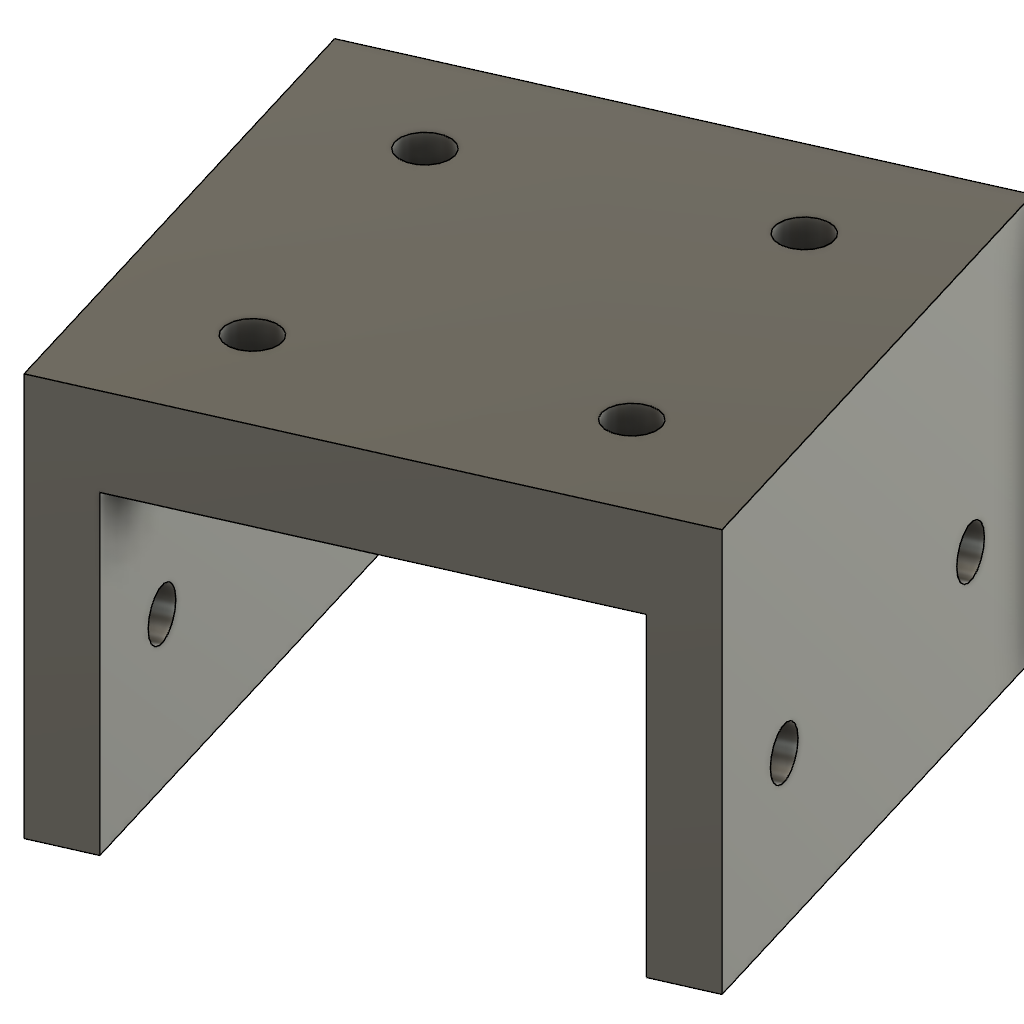
\includegraphics[width=0.8\linewidth]{figures/hardware_design/turret_clamp.png}
        \caption{Laser turret clamp.}
    \end{subfigure}
    \quad
    \begin{subfigure}{0.45\textwidth}
        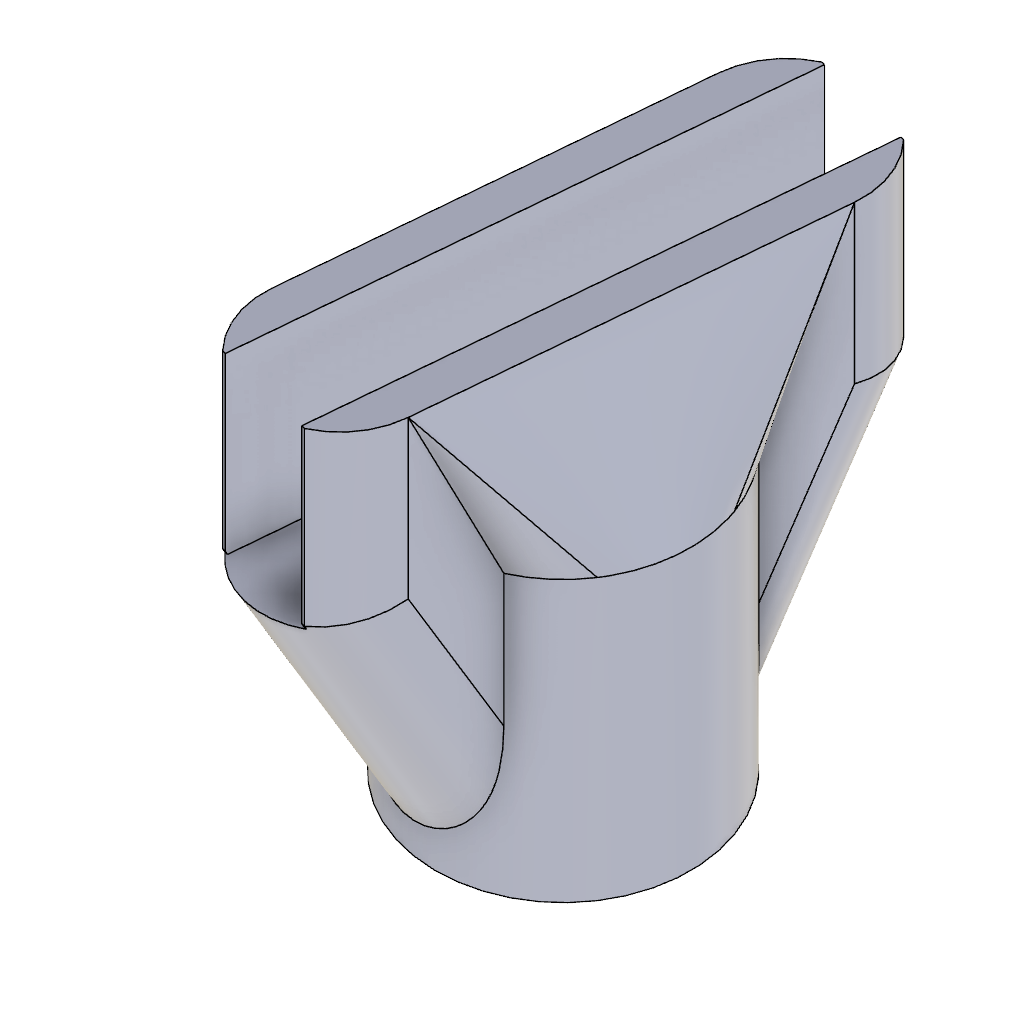
\includegraphics[width=0.8\linewidth]{figures/hardware_design/mirror_holder.png}
        \caption{Mirror holder.}
    \end{subfigure}
    \caption{Laser turret subcomponents.}
    \label{fig:turret_subcomponents}
\end{figure}



\FloatBarrier
\subsection{Software design}
\textit{Mapping between pixels and real distance. Mosquito detection and tracking. Laser detection and tracking. \gls{pid} controller. Feedback for turret. Distinguishing between laser reflections.}



\subsubsection{Mosquito and laser detection} \label{subsubsec:mosquito_and_laser_detection}
It was assumed that the mosquitoes would be the only dark blobs in the enclosure and that the laser and its reflections would be the only bright blobs in the enclosure. The video frame will be cropped such that only the white back surface of the enclosure is visible. To reduce the computational complexity of the image processing only the red channel of the \gls{rgb} frame will be used, hence, the necessity of the red laser.

The mosquito detection was designed to detect dark blobs in the enclosure and would not be able to distinguish between mosquitoes and other dark blobs. The laser detection was designed to detect bright blobs in the enclosure and would not be able to distinguish between the laser's reflections and other bright blobs. The mosquito and laser detection processes are similar in nature. The basic detection process flow is shown in \autoref{fig:detection_process_flow}.
\begin{figure}[h]
    \centering
    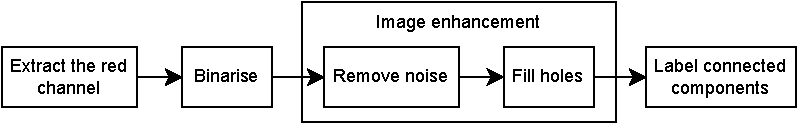
\includegraphics[width=\textwidth]{figures/detection/detection_process_flow.pdf}
    \caption{Detection process flow.}
    \label{fig:detection_process_flow}
\end{figure}
The red channel of the \gls{rgb} frame will be extracted, which will be referred to as the frame for the rest of this discussion. The difference between the mosquito and laser detection occurs in the binarisation step. A copy of the frame is made before binarising so that both the mosquito and laser detection can be performed since the frame will be overwritten in the image processing steps in pursuit of efficiency.


\paragraph{Binarisation}\mbox{}\\
The frame will be binarised using a threshold value. The exposure of the camera will be fixed and the lighting in the mosquito enclosure will be controlled thus the threshold value will be fixed. To detect mosquitoes the frame will be binarised with a less than threshold since the mosquitoes will be darker than the white background. To detect the laser's reflections the frame will be binarised with a greater than threshold since the laser and its reflections will be brighter than the white background. The ideal result of the binarisation is an image where the mosquitoes and the laser's reflections are the only foreground pixels in their respective copies of the frame. This will not be the case since the mosquitoes and the laser's reflections can not be perfectly isolated using a threshold value in frame that will contain noise from the camera sensor.


\paragraph{Image enhancement}\mbox{}\\
The binarised frames are subject to noise, holes, and erroneously joint or disjointed sections. This can be resolved using morphological operations.
The goal of the morphological operations is to ensure that all the foreground pixels that correspond to a detection are connected, that there are no foreground pixels that do not correspond to a detection, and that there are no erroneously joint or disjoint foreground pixels. There must be a one to one correspondence between the groups of connected foreground pixels and the objects that must be detected. The connectivity of pixels will be explained in \autoref{par:ccl}. Morphological operations work by passing a structuring element over the pixels in an image and performing a logical operation on the pixels in the image that are covered by the structuring element.

The noise and erroneously joint sections are removed using the morphological opening operation. Opening has been formally defined in \autoref{subsubsec:morphological_operations}. The opening of $A$ by $B$ is the union of all translations of $B$ that are completely contained in $A$ as illustrated in \autoref{fig:opening}. The holes and erroneously disjointed sections are removed using the morphological closing operation. Closing has been formally defined \autoref{subsubsec:morphological_operations}. The closing of $A$ by $B$ is the complement of the union of all translations of $B$ that do not overlap $A$ as illustrated in \autoref{fig:closing}.

The structuring element must be identical independent of orientation in a 2D image since the orientation of the mosquitoes will be unknown. The structuring element will therefore be a disc. The size of the disc will be adjusted independently for the opening and closing operations for both the mosquito and laser detection.


\paragraph{Connected components labelling}\label{par:ccl}\mbox{}\\
From the enhanced binary frames the co-ordinates of the connected foreground pixels must be obtained. This is done using \gls{ccl}. \Gls{ccl} is the process of assigning a label to each foreground pixel in a binary image such that connected pixels have the same label. The connectivity of pixels are defined using either four or eight connectivity. Four connectivity defines the neighbourhood of a pixel as the pixels to the left, right, top, and bottom of the pixel. Eight connectivity defines the neighbourhood of a pixel as the pixels to the left, right, top, bottom, top left, top right, bottom left, and bottom right of the pixel. The \gls{ccl} connectivity is shown in \autoref{fig:ccl_connectivity}.
\begin{figure}[h]
    \centering
    \begin{subfigure}[b]{0.3\textwidth}
        \centering
        % 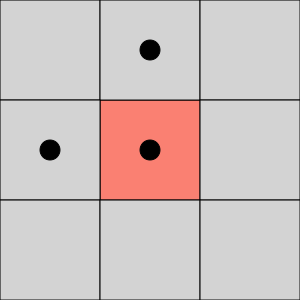
\includegraphics[width=0.5\linewidth]{figures/detection/square_4_connectivity.png}
        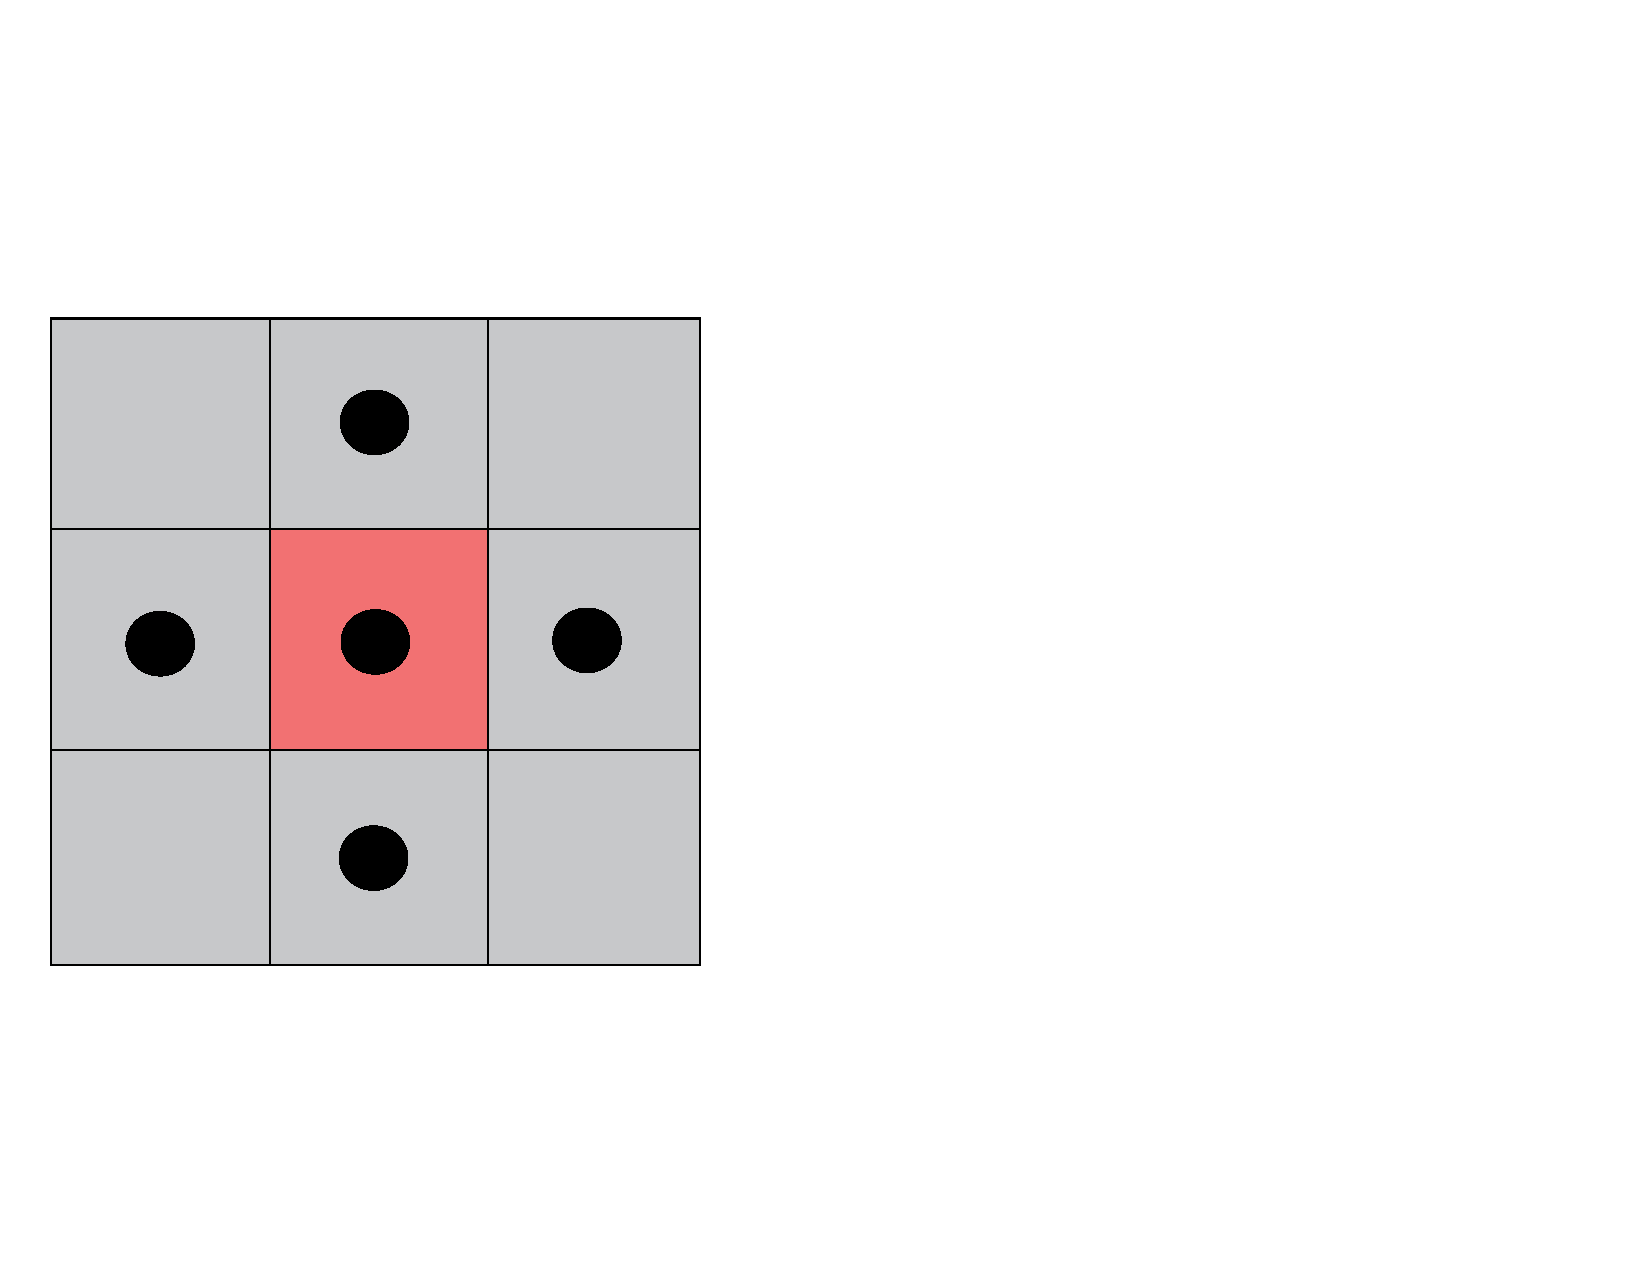
\includegraphics[width=0.6\linewidth]{figures/detection/4_pixel_connectivity.pdf}
        \caption{Four connectivity.}
        \label{fig:four_connectivity}
    \end{subfigure}
    \quad
    \begin{subfigure}[b]{0.3\textwidth}
        \centering
        % 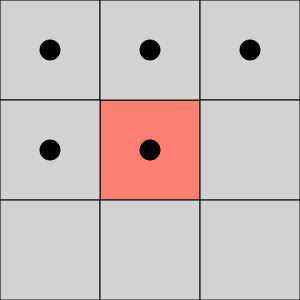
\includegraphics[width=0.5\linewidth]{figures/detection/square_8_connectivity.png}
        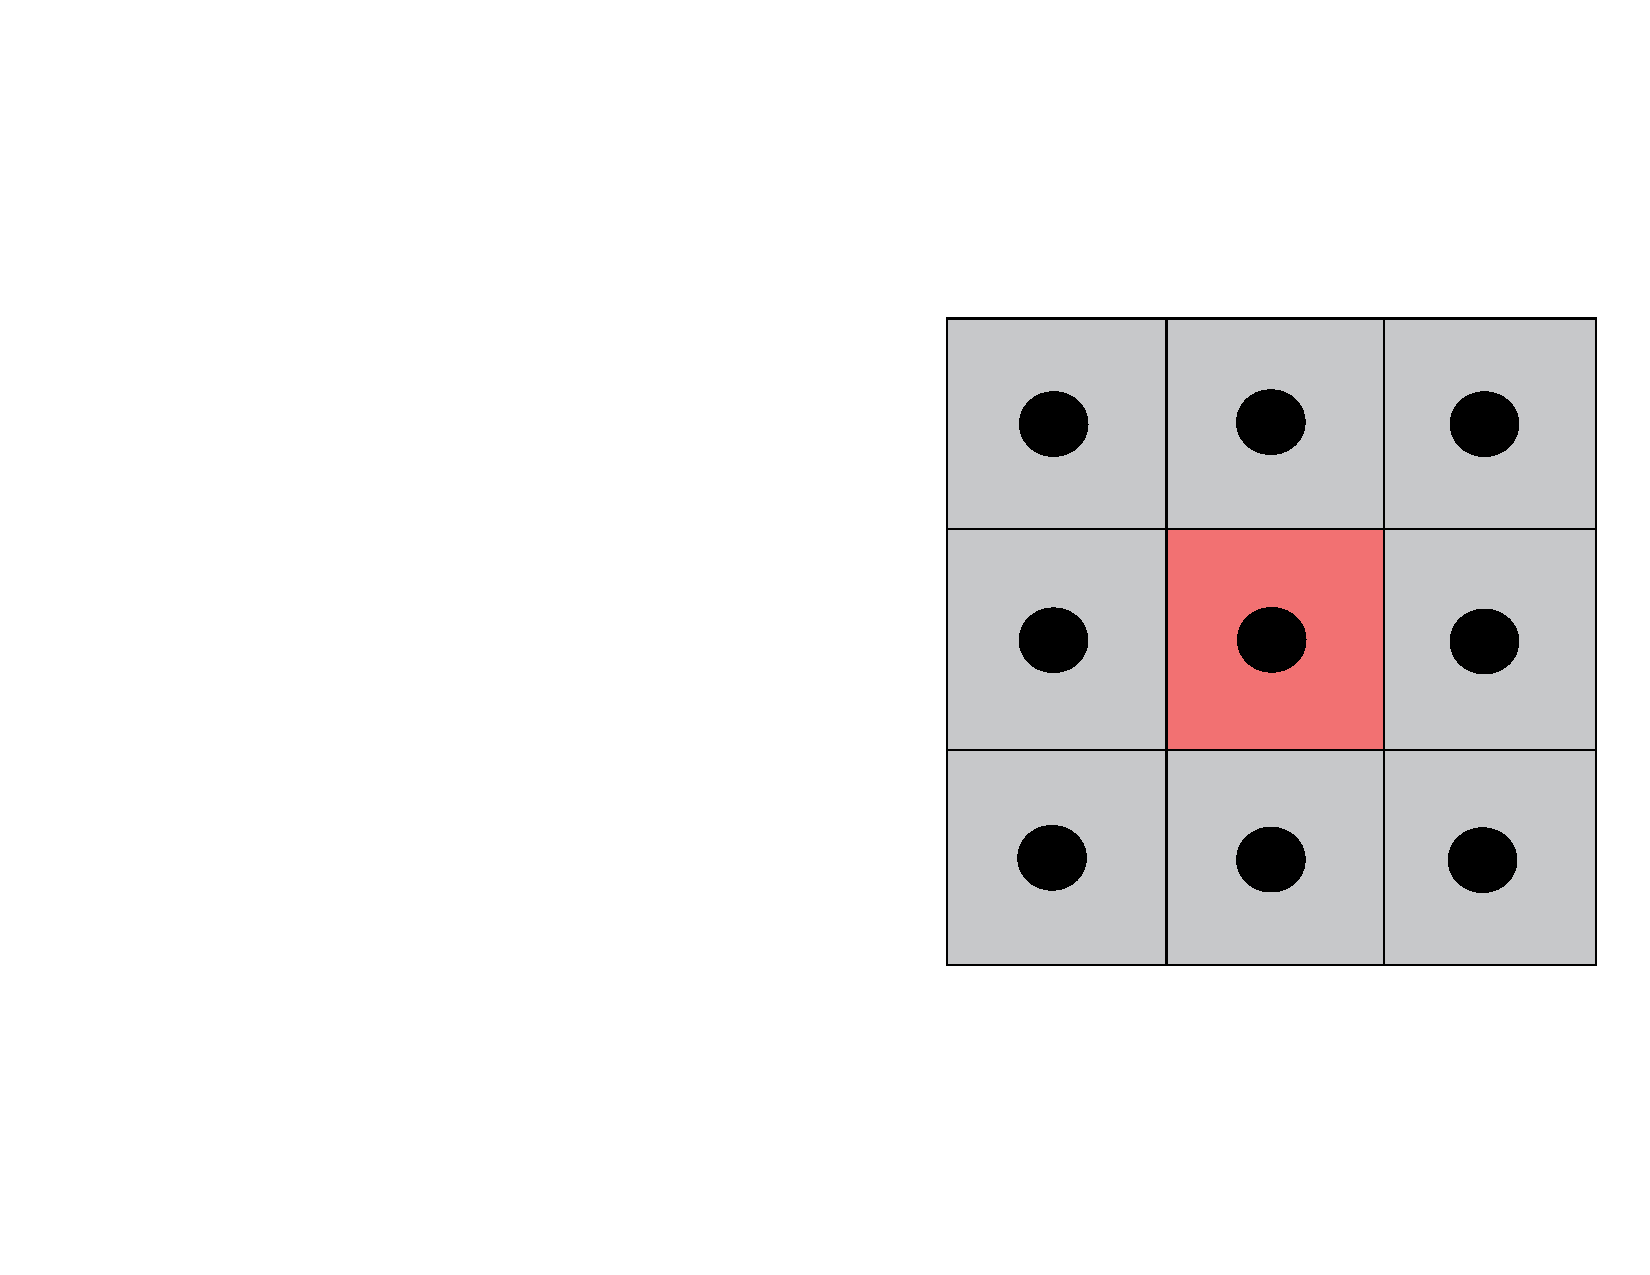
\includegraphics[width=0.6\linewidth]{figures/detection/8_pixel_connectivity.pdf}
        \caption{Eight connectivity.}
        \label{fig:eight_connectivity}
    \end{subfigure}
    \caption{Connected components labelling connectivity.}
    \label{fig:ccl_connectivity}
\end{figure}

Various algorithms exist to perform \gls{ccl}. Two of the most commonly used algorithms are the two-pass algorithm and the breadth-first single-pass algorithm. The two-pass algorithm is generally faster for images with large connected components and the breadth-first single-pass algorithm is generally faster for images with small connected components. The nature of the mosquito and laser detection is such that the connected components will be small, thus the breadth-first single-pass algorithm was chosen. The breadth-first single-pass algorithm is presented in \autoref{alg:single_pass_ccl}.
\begin{algorithm}[h]
    \caption{Breadth-First Single-Pass Connected Component Labelling}
    \label{alg:single_pass_ccl}
    \begin{algorithmic}[1]
        \Procedure{SinglePassCCL}{$image$}
        \State $rows, cols \gets \text{dimensions of } image$
        \State $label \gets 1$
        \State $labels \gets \text{2D array of zeros of size } rows \times cols$
        \For{$y \gets 0$ to $rows-1$}
        \For{$x \gets 0$ to $cols-1$}
        \If{$image[y][x] = 1$ and $labels[y][x] = 0$}
        \State $\text{ExploreBlob}(image, labels, x, y, label)$
        \State $label \gets label + 1$
        \EndIf
        \EndFor
        \EndFor
        \EndProcedure
        \State
        \Procedure{ExploreBlob}{$image, labels, x, y, label$}
        \State $queue \gets \text{empty queue}$
        \State $\text{Enqueue}(queue, (x, y))$
        \While{$\text{not empty}(queue)$}
        \State $(x, y) \gets \text{Dequeue}(queue)$
        \If{$x < 0$ or $x \geq cols$ or $y < 0$ or $y \geq rows$ or $image[y][x] = 0$ or $labels[y][x] > 0$}
        \State \text{continue}
        \EndIf
        \State $labels[y][x] \gets label$
        \For{each neighbor $(nx, ny)$ of $(x, y)$}
        \State $\text{Enqueue}(queue, (nx, ny))$
        \EndFor
        \EndWhile
        \EndProcedure
    \end{algorithmic}
\end{algorithm}



\subsubsection{Distinguishing between the laser's reflections}
The laser must shine through the front glass of the mosquito enclosure. This results in various reflections of the laser beam. There are three predominate reflections that can not be distinguished using a brightness threshold. These reflections are:
\begin{itemize}
    \item The reflection of the laser beam off the front glass at the origin of the laser turret, resulting from scattered light off the turret mirrors.
    \item The reflection of the laser beam incident on the front glass.
    \item The reflection of interest, which is the reflection of the laser beam incident on a mosquito or the back surface of the enclosure.
\end{itemize}

The reflection off the front glass at the origin of the laser turret remains stationary since the laser turret itself is stationary with only the angles of the mirrors changing. The remaining two reflections are distinguished using the geometric properties of the system positioning. The $yz$-plane of the system is shown in \autoref{fig:distinguish_lasers}. The laser turret is slightly below the camera which is exaggerated in \autoref{fig:distinguish_lasers} for illustration purposes. It can be seen in \autoref{fig:distinguish_lasers} that if both detections are at or below the camera origin the reflection of interest is closer to the camera origin. If both reflections are at or above the camera origin then the reflection of interest is further from the camera origin. If the reflections are on either side of the camera origin the reflection of interest is the reflection above the camera origin. This logic is easily extended to three dimensions by considering the $yz$-plane and $xz$-plane independently.
\begin{figure}[h]
    \centering
    \begin{subfigure}[t]{0.45\textwidth}
        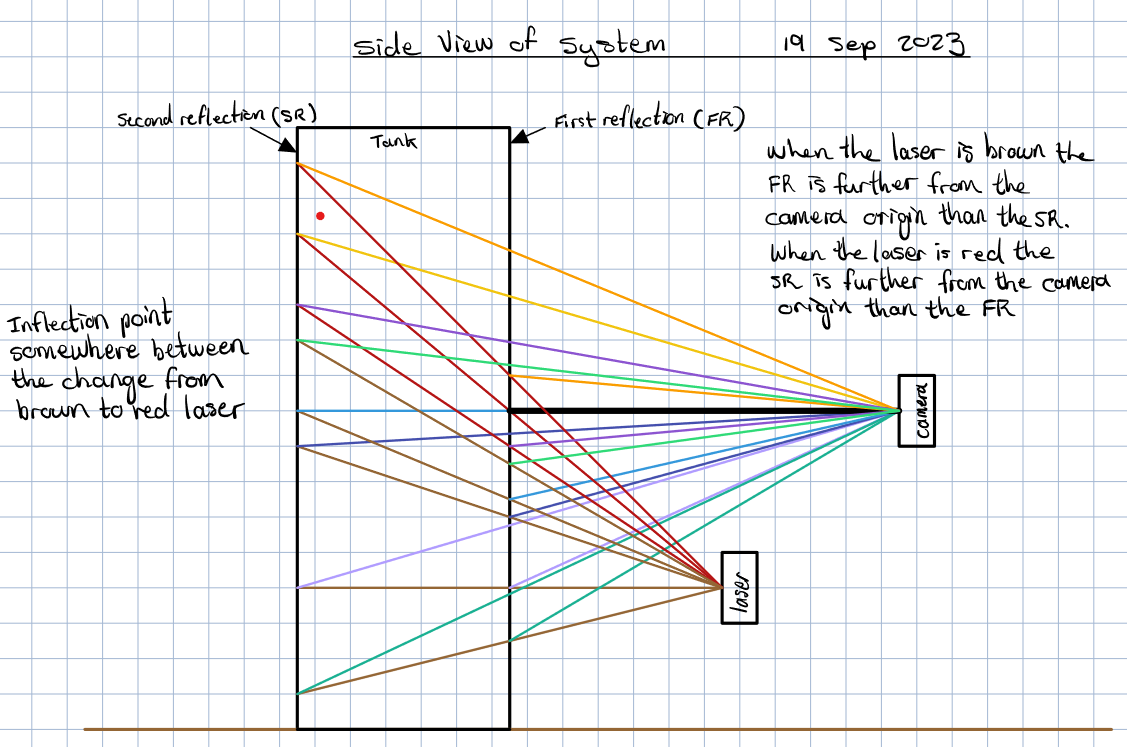
\includegraphics[width=\linewidth]{figures/distinguish_lasers.png}
        \caption{Laser reflections.}
    \end{subfigure}
    \quad
    \begin{subfigure}[t]{0.45\textwidth}
        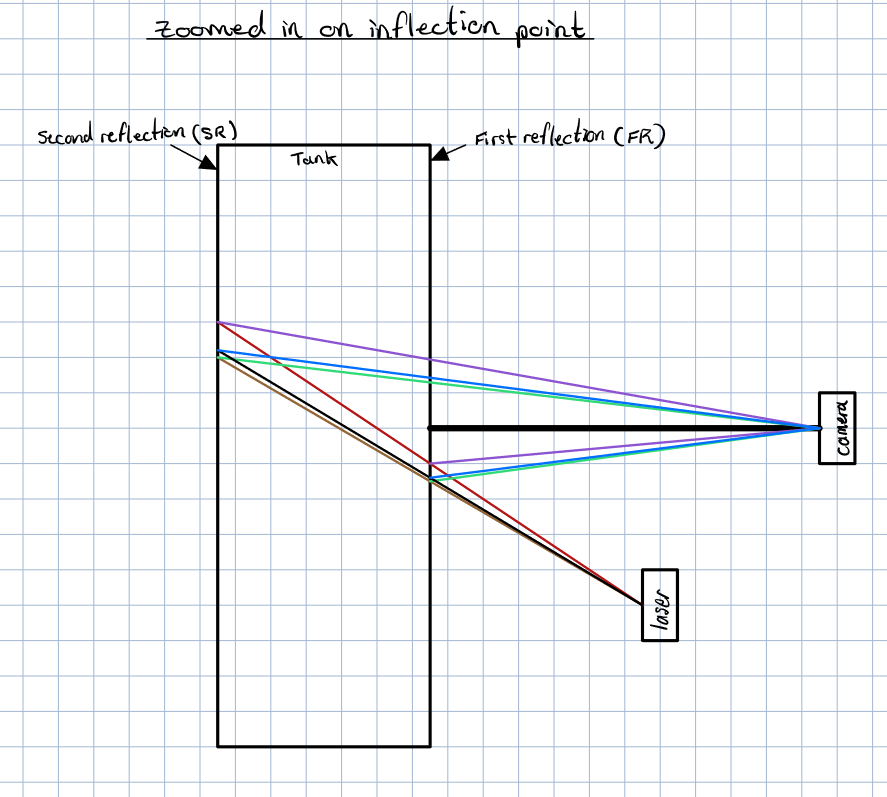
\includegraphics[width=\linewidth]{figures/distinguish_lasers_zoomed_inflection.png}
        \caption{Laser reflections zoomed in on the inflection point.}
    \end{subfigure}
    \caption{Distinguishing between the laser's reflections.}
    \label{fig:distinguish_lasers}
\end{figure}



\subsubsection{Mosquito tracking}
The mosquito tracking was performed using the \gls{sort} algorithm. The \gls{sort} algorithm is based on the tracking-by-detection paradigm, which means it relies on an external object detector. The object detector used was the mosquito detection algorithm described in \autoref{subsubsec:mosquito_and_laser_detection}. The \gls{sort} algorithm associates the detections across frames to create tracks.


\paragraph{Tracks}\mbox{}\\
The mosquito tracks are created using the Kalman filter. The theoretical background of Kalman filter is discussed in \autoref{subsubsec:kalman_filter}. The kinematic equation representing the flight of a mosquito must be defined to determine the state space of the Kalman filter. The kinematic equation used to model the flight of a mosquito is
\begin{equation}
    \label{eq:mosquito_kinematic_equation}
    \mathbf{x}_{k} = \mathbf{x}_{k-1} + \mathbf{\dot{x}}_{k-1}\Delta t + \frac{1}{2}\mathbf{\ddot{{x}}}_{k-1}\Delta t^2\,,
\end{equation}
where $\mathbf{x}_{k}$ is the position vector defined by the 2D pixel co-ordinate of a mosquito $\begin{bmatrix} x & y \end{bmatrix}^\mathrm{T}$. A constant velocity model with acceleration as noise will be used since mosquitoes have an erratic flight pattern. Therefore, the set of differential equations describing the state space of the Kalman filter is
\begin{equation}
    \begin{split}
        \mathbf{x}_k
        & = \mathbf{Ax}_{k-1} + \mathbf{Bu}_k + \mathbf{w}_k \\
        \begin{bmatrix}
            x_k       \\
            y_k       \\
            \dot{x}_k \\
            \dot{y}_k
        \end{bmatrix}
        & =
        \begin{bmatrix}
            1 & 0 & \Delta t & 0        \\
            0 & 1 & 0        & \Delta t \\
            0 & 0 & 1        & 0        \\
            0 & 0 & 0        & 1
        \end{bmatrix}
        \begin{bmatrix}
            x_{k-1}       \\
            y_{k-1}       \\
            \dot{x}_{k-1} \\
            \dot{y}_{k-1}
        \end{bmatrix}\,,
    \end{split}
\end{equation}
where $\mathbf{u}_k$ is the input vector, which is the acceleration of the mosquito according to its kinematic flight model defined in \autoref{eq:mosquito_kinematic_equation}. However, this acceleration is unknown and will be compensated for by the process noise $\mathbf{w}_k$, thus $\mathbf{u}_k = \mathbf{0}$. The process noise $\mathbf{w}_k$ is assumed to be drawn from a zero mean multivariate normal distribution $\mathcal{N}$ with covariance $\mathbf{Q}_k$. Hence, $\mathbf{w}_k \sim$ $\mathcal{N}$ $\left(0, \mathbf{Q}_k\right)$, thus, $\mathbb{E}[w_k] = 0$ and $\mathbb{E}[w_kw_k^\mathrm{T}] = \mathbf{Q}_k$. The process noise covariance matrix $\mathbf{Q}$ is given by
\begin{equation}
    \label{eq:kalman_filter_process_noise_covariance_matrix}
    \mathbf{Q} = \begin{bmatrix}
        \sigma_{x}^2               & 0                          & \sigma_{x}\sigma_{\dot{x}} & 0                          \\
        0                          & \sigma_{y}^2               & 0                          & \sigma_{y}\sigma_{\dot{y}} \\
        \sigma_{\dot{x}}\sigma_{x} & 0                          & \sigma_{\dot{x}}^2         & 0                          \\
        0                          & \sigma_{\dot{y}}\sigma_{y} & 0                          & \sigma_{\dot{y}}^2
    \end{bmatrix}\,,
\end{equation}
where $\sigma_{x}$ and $\sigma_{\dot{x}}$ are the standard deviations of the position and velocity, respectively. The standard deviation of the position is defined as the standard deviation of the acceleration $\sigma_{\ddot{x}}$ multiplied by $\frac{1}{2}\Delta t^2$ since this is the effect that the acceleration will have on the position as shown in \autoref{eq:mosquito_kinematic_equation}. Similarly, the standard deviation of the velocity is defined as $\Delta t \sigma_{\ddot{x}}$. Therefore, the process noise covariance can be written as
\begin{equation}
    \mathbf{Q} =
    \sigma_{\ddot{x}}^{2}
    \begin{bmatrix}
        \frac{\Delta t^4}{4} & 0                    & \frac{\Delta t^3}{2} & 0                    \\
        0                    & \frac{\Delta t^4}{4} & 0                    & \frac{\Delta t^3}{2} \\
        \frac{\Delta t^3}{2} & 0                    & \Delta t^2           & 0                    \\
        0                    & \frac{\Delta t^3}{2} & 0                    & \Delta t^2
    \end{bmatrix}\,.
\end{equation}

The position of a mosquito is the only component of the state that is measured by the detection system. Thus, the observation matrix $\mathbf{H}$ is
\begin{equation}
    \mathbf{H} = \begin{bmatrix}
        1 & 0 & 0 & 0 \\
        0 & 1 & 0 & 0
    \end{bmatrix}\,.
\end{equation}
The measurement noise covariance matrix $\mathbf{R}$ is
\begin{equation}
    \mathbf{R} = \begin{bmatrix}
        \sigma_{x}^2 & 0            \\
        0            & \sigma_{y}^2
    \end{bmatrix}\,,
\end{equation}
where $\sigma_{x}^2$ and $\sigma_{y}^2$ are the variances of the position detected. The initial state covariance matrix $\mathbf{P}$ is given by
\begin{equation}
    \mathbf{P} = \begin{bmatrix}
        \sigma_{x}^2 & 0            & 0               & 0               \\
        0            & \sigma_{y}^2 & 0               & 0               \\
        0            & 0            & \dot{x}_{max}^2 & 0               \\
        0            & 0            & 0               & \dot{y}_{max}^2
    \end{bmatrix}\,.
\end{equation}

The Kalman filter is initialised with the position of the mosquito as the initial state $\mathbf{x}_0$. The position of the mosquito in the next frame $\mathbf{\hat{x}}_{k\mid k-1}$ is predicted using the adapted predict equation of the Kalman filter $\mathbf{\hat{x}}_{k\mid k-1} = \mathbf{A}_k \mathbf{x}_{k-1\mid k-1}$. This prediction will be used in the association step before the update step. The update step of the Kalman filter is performed using the update equation of the Kalman filter $\mathbf{x}_{k\mid k} = \mathbf{x}_{k\mid k-1} + \mathbf{K}_k \left(\mathbf{z}_k - \mathbf{H}_k \mathbf{x}_{k\mid k-1}\right)$, where $\mathbf{K}_k$ is the Kalman gain and $\mathbf{z}_k$ is the measurement vector. The measurement vector $\mathbf{z}_k$ is the position of the mosquito detected in the current frame.


\paragraph{Association}\mbox{}\\
The association of tracks and detections will be done using the Hungarian algorithm, which is an optimised optimal assignment algorithm. The Hungarian algorithm has a time complexity of $O\left(n!\right)$ compared to the time complexity na\"ive approach $O\left(n^3\right)$. The Hungarian algorithm works as follows:
\begin{description}[style=nextline]
    \item[Generate a cost matrix.] Represent the problem with a square $n \times n$ matrix $\mathbf{C}$ where the element $\mathbf{C}_{i,j}$ represents the cost of assigning track $i$ to detection $j$. The cost function is the euclidean distance between the predicted location and the detected location of the mosquito.
    \item[Row and column reduction.] Subtract the minimum value in each row from each element in the row. Perform the same operation for each column. This will produce a matrix with at least one zero in each row and column.
    \item[Cover zeros and check for optimality.] Cover all the zeros in the matrix using the minimum number of horizontal and vertical lines. If the minimum number of covering lines is $n$, an optimal assignment exists among the zeros, and the algorithm can proceed to the assignment phase. If not, you need to adjust the matrix and repeat from this step.
    \item[Adjust the matrix.] Find the smallest element that is not covered by any line. Subtract this element from all uncovered elements, and add it to all elements at the intersections of the covering lines. Return to \textit{cover zeros and check for optimality}.
    \item[Assignment.] Once an optimal assignment is found, read the assignment from the zeros in the matrix. \sout{Each row will have exactly one zero, and each column may have one zero. If a column has no zeros, the track corresponding to that column is unassigned. If a column has more than one zero, the track corresponding to that column is assigned to the detection corresponding to the zero that is covered by a star. If a row has more than one zero, the track corresponding to that row is assigned to the detection corresponding to the zero that is covered by a star.}
\end{description}



\subsubsection{Laser turret control system}
The laser turret control system is a closed-loop \gls{pid} controller. A \gls{pid} controller is represented by the following equation
\begin{equation}
    \label{eq:pid_controller}
    u(t) = K_p e(t) + K_i \int_{0}^{t} e(\tau) d\tau + K_d \frac{de(t)}{dt}\,,
\end{equation}
where $u(t)$ is the control signal, $e(t)$ is the error signal, $K_p$ is the proportional gain, $K_i$ is the integral gain, and $K_d$ is the derivative gain. The goal of the laser turret control system is to position the laser beam at the target co-ordinates. The target co-ordinates is defined by the mosquito detection and tracking system in pixels. The stepper motors are controlled in steps, thus the target pixels and must be mapped to the number of steps required to move the laser beam to the target co-ordinates. The steps are defined in reference to the origin of the laser defined in \autoref{subsubsec:laser_turret_design}, which is the position when the laser beam is perpendicular to the $xy$-plane of the mosquito enclosure. The block diagram of the laser turret control system can be seen in \autoref{fig:control_system}. The two axes of the laser turret are controlled independently each having their own \gls{pid} controller. The \gls{pid} controller is implemented in software and the control signal is sent to the stepper motor drivers using \gls{gpio}.
\begin{figure}[h]
    \centering
    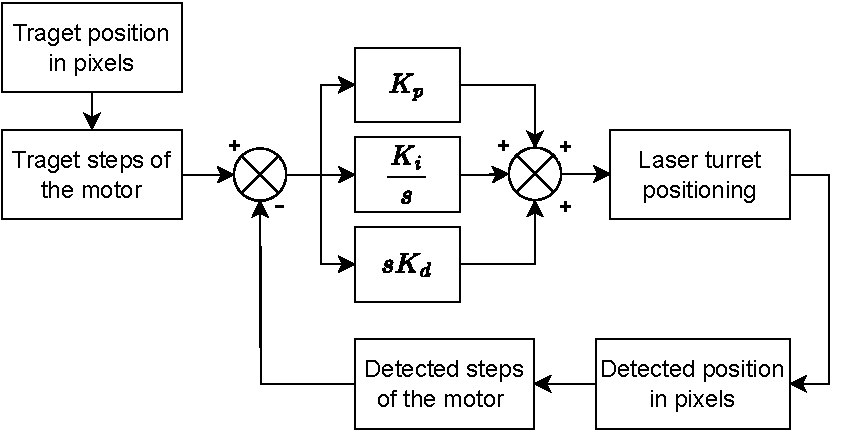
\includegraphics[width=0.8\textwidth]{figures/control_system.pdf}
    \caption{Laser turret control system.}
    \label{fig:control_system}
\end{figure}



\subsection{Software implementation and optimisation}
Only using red channel, \gls{gpu}, low resolution, etc.
\gls{gpio} interfacing with stepper motor driver.

The Raspberry Pi camera v2 was chosen. The low resolution was 700 x 300 was chosen to reduce computational complexity.

\subsubsection{Image processing}
The binarisation and image enhancement processes described in \autoref{subsubsec:mosquito_and_laser_detection} are suitable for parallelisation. Therefore, custom \gls{cuda} kernels were written to perdform these operations on \gls{gpu}.

\begin{minipage}{\linewidth}
    \begin{lstlisting}[language=C++, caption={Erosion GPU kernel.}]
__global__ void erosion(uint8_t* input,
                        uint8_t* output,
                        uint8_t* struct_elem,
                        int struct_elem_radius) {
  int x = blockIdx.x * blockDim.x + threadIdx.x;
  int y = blockIdx.y * blockDim.y + threadIdx.y;
  
  if (x < d_COLS && y < d_ROWS) {
    int min_val = 255;
    for (int i = -struct_elem_radius; i <= struct_elem_radius; i++) {
      for (int j = -struct_elem_radius; j <= struct_elem_radius; j++) {
        if (y + i >= 0 && y + i < d_ROWS && x + j >= 0 && x + j < d_COLS) 
        {
          if (struct_elem[(i + struct_elem_radius) *
                          (2 * struct_elem_radius + 1) +
                          j + struct_elem_radius] == 1) 
          {
            int idx = (y + i) * d_COLS + (x + j);
            min_val = min(min_val, (int)input[idx]);
          }
        }
      }
    }
    output[y * d_COLS + x] = min_val;
  }
}
\end{lstlisting}
\end{minipage}



\subsubsection{Laser turret control}
The laser turret control consists of various independent subcomponents that required meticulous attention to detail to successfully integrate. The integration will be discussed in \autoref{subsec:integration}. The focus in this section will be on the subcomponents.


\paragraph{Interfacing with stepper motor drivers}\mbox{}\\
The stepper motors drivers were connected to the Nvidia Jetson Nano \gls{gpio} according to the diagram in \autoref{fig:stepper_driver_pins}.
\begin{figure}
    \centering
    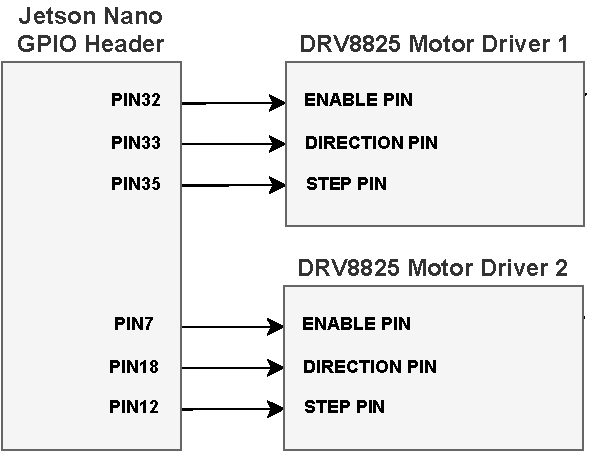
\includegraphics[width=0.6\textwidth]{figures/stepper_driver_pins.pdf}
    \caption{Stepper motor driver connections.}
    \label{fig:stepper_driver_pins}
\end{figure}
The motors are enabled by setting the \texttt{ENABLE PIN} to a logical high. The direction of rotation is determined by the logic level of the \texttt{DIRECTION PIN}. The stepper motors are driven by pulsing the \texttt{STEP PIN} at the desired frequency for the desired number of steps.
\begin{algorithm}[h]
    \caption{Stepper Motor Control}
    \label{alg:stepper_control}
    \begin{algorithmic}[1]
        \State $ENABLE\;PIN \gets \text{logical high}$
        \State $DIRECTION\;PIN \gets direction$
        \For{$step \gets 0$ to $steps-1$}
        \State $STEP\;PIN \gets \text{logical high}$
        \State $\text{delay}(period)$
        \State $STEP\;PIN \gets \text{logical low}$
        \State $\text{delay}(period)$
        \EndFor
    \end{algorithmic}
\end{algorithm}


\paragraph{Converting pixels to steps}\mbox{}\\
The laser turret control system must be able to position the laser beam at any pixel in the enclosure. The laser turret control system must therefore be able to convert pixels to steps. The conversion from pixels to steps is done using the following equation
\begin{equation}
    \label{eq:pixels_to_steps}
    \text{steps} = \frac{\text{pixels}}{\text{pixels per step}}\,,
\end{equation}



\subsection{Final system integration and testing}\label{subsec:integration}
Real-time multi threading.

\newpage

%% End of File.

